\section{Example Cases}
\subsection{Convection in 2D Annulus}
We consider a natural convection between the two concentric cylinders as
considered by Grigull \& Hauf and presented by Van Dyke. The inner cylinder
(diameter $D$) is slightly heated with with respect to the outer one (diameter
$3D$). The Boussinesq approximation is used to formulate the equations of
motion, valid in situations where density differences are small enough to be
neglected everywhere except in the gravitational forcing.  
Normalizing the Navier-Stokes and energy equations with $D$ for the length
scale and $D/U$ for the time scale ($U \approx \sqrt{\alpha g D (T_1-T_0)}$) is
the characteristic velocity in the given problem), and introducing
nondimensional temperature $\theta=(T-T_0)/(T_1-T_0)$, where $T_0$ and $T_1$
are the respective temperatures of the outer and inner cylinders, the governing
equations take the nondimensional form
\begin{align}
   \pp{\bu}{t} + \bu \cdot \nabla \bu & = -\nabla p + \frac{1}{\sqrt{Gr}}
\nabla^2 \bu + \theta, \quad \nabla \bu = 0, \\ \pp{\theta}{t} + \bu \cdot
\nabla \theta & = \frac{1}{\sqrt{Gr}Pr} \nabla^2 \theta.
\end{align}
Here $\bu$ is the velocity vector, $p$ is the pressure, $\theta$ is the
temperature.  The Grashof and Prandtl numbers are defined as
\begin{equation}
   {\rm Gr} = \frac{\alpha g (T_1-T_0) D^3}{\nu^2}, \quad {\rm Pr} =
\frac{\nu}{\alpha},
\end{equation}
where $\nu$ is the kinematic viscosity, $\alpha$ is the volumetric thermal
expansion coefficient, and $g$ is the acceleration due to gravity. 

For $\rm Gr \in [\num{3e+05},~\num{9e+05}]$, the solution is steady; a
steady-state solution is obtained when the change in velocity magnitude
$\approx 10^{-7}$ between successive time steps.  Fig.~\ref{fig:1}, we show the
change in velocity magnitude between successive time steps at multiple $\rm
Gr$. As expected, as $\rm Gr$ increases, it takes more time for the solution to
reach its steady state.
\begin{figure}[!h]
     \centering
     \includegraphics[width=\textwidth]{/Users/bigticket0501/NekMOR_cases/annulus_2d/study_acceleration/dvdt_gr}
     \caption{Change in velocity magnitude between successive time steps at
     multiple $\rm Gr$.} \label{fig:1}
\end{figure}

\subsubsection{Acceleration to steady state with ROM}
Next we would like to study if the ROM is able to accelerate the process to
reach the steady state.  

Given a tolerance $\text{tol}$, we first run the FOM until the criterion
$\|\bu^i - \bu^{i-1}\|_\infty / \Delta t < \text{tol}$ is meet. We then collect
the last five snapshots and build the ROM. We then run the ROM for $t=2000(s)$
and restart the FOM with the ROM solution.

Fig.~\ref{fig:2_a} shows the behavior of the change in velocity magnitude between
successive time steps in FOM at $\rm Gr=\num{3e+05}$ with three thresholds
$\text{tol}=10^{-2},~10^{-3},~10^{-4}$.  

Fig.~\ref{fig:2_b} shows the performance of the same quantities at $\rm
Gr=\num{9e+05}$. Note that the last ten snapshots are used to build the ROM in
this case.

\begin{figure}[!h]
     \centering
     \begin{subfigure}[b]{0.45\textwidth}
         \centering
         \includegraphics[width=\textwidth]{/Users/bigticket0501/NekMOR_cases/annulus_nekrom/post_process/Gr3E+05_lx10/std_dvdt_Gr300000}
         \caption{$\rm Gr=\num{3e+05}$, $lx1=10$}
         \label{fig:2_a}
     \end{subfigure}
     \hfill
     \begin{subfigure}[b]{0.45\textwidth}
         \centering
         \includegraphics[width=\textwidth]{/Users/bigticket0501/NekMOR_cases/annulus_nekrom/post_process/Gr9E+05_lx10/std_dvdt_Gr900000}
         \caption{$\rm Gr=\num{9e+05}$, $lx1=10$}
         \label{fig:2_b}
     \end{subfigure}\\
     \begin{subfigure}[b]{0.45\textwidth}
         \centering
         \includegraphics[width=\textwidth]{/Users/bigticket0501/NekMOR_cases/annulus_nekrom/post_process/Gr3E+05_lx12/std_dvdt_Gr300000}
         \caption{$\rm Gr=\num{3e+05}$, $lx1=12$}
         \label{fig:2_c}
     \end{subfigure}
     \hfill
     \begin{subfigure}[b]{0.45\textwidth}
         \centering
         \includegraphics[width=\textwidth]{/Users/bigticket0501/NekMOR_cases/annulus_nekrom/post_process/Gr9E+05_lx12/std_dvdt_Gr900000}
         \caption{$\rm Gr=\num{9e+05}$, $lx1=12$}
         \label{fig:2_d}
     \end{subfigure}
     \caption{
     \subref{fig:2_a}--\subref{fig:2_b}: Behavior of the change in velocity magnitude
     between successive time steps in FOM at $\rm Gr=\num{3e+05}$ and $\rm
     Gr=\num{9e+05}$ with $lx1=10$.
     \subref{fig:2_c}--\subref{fig:2_d}: Performance of the same quantities
     with $lx1=12$.  The FOM was run with different initial conditions
     $\chi_n$, corresponding to the ROM solutions approximated with RB space
     generated with snapshots collected before
     $\|\bu^i-\bu^{i-1}\|_{\infty}/\Delta t < 1e^{-n}$.} \label{fig:2}
\end{figure}

\subsubsection{pMOR}
\begin{figure}[!h]
     \centering
     \begin{subfigure}[b]{0.45\textwidth}
         \centering
         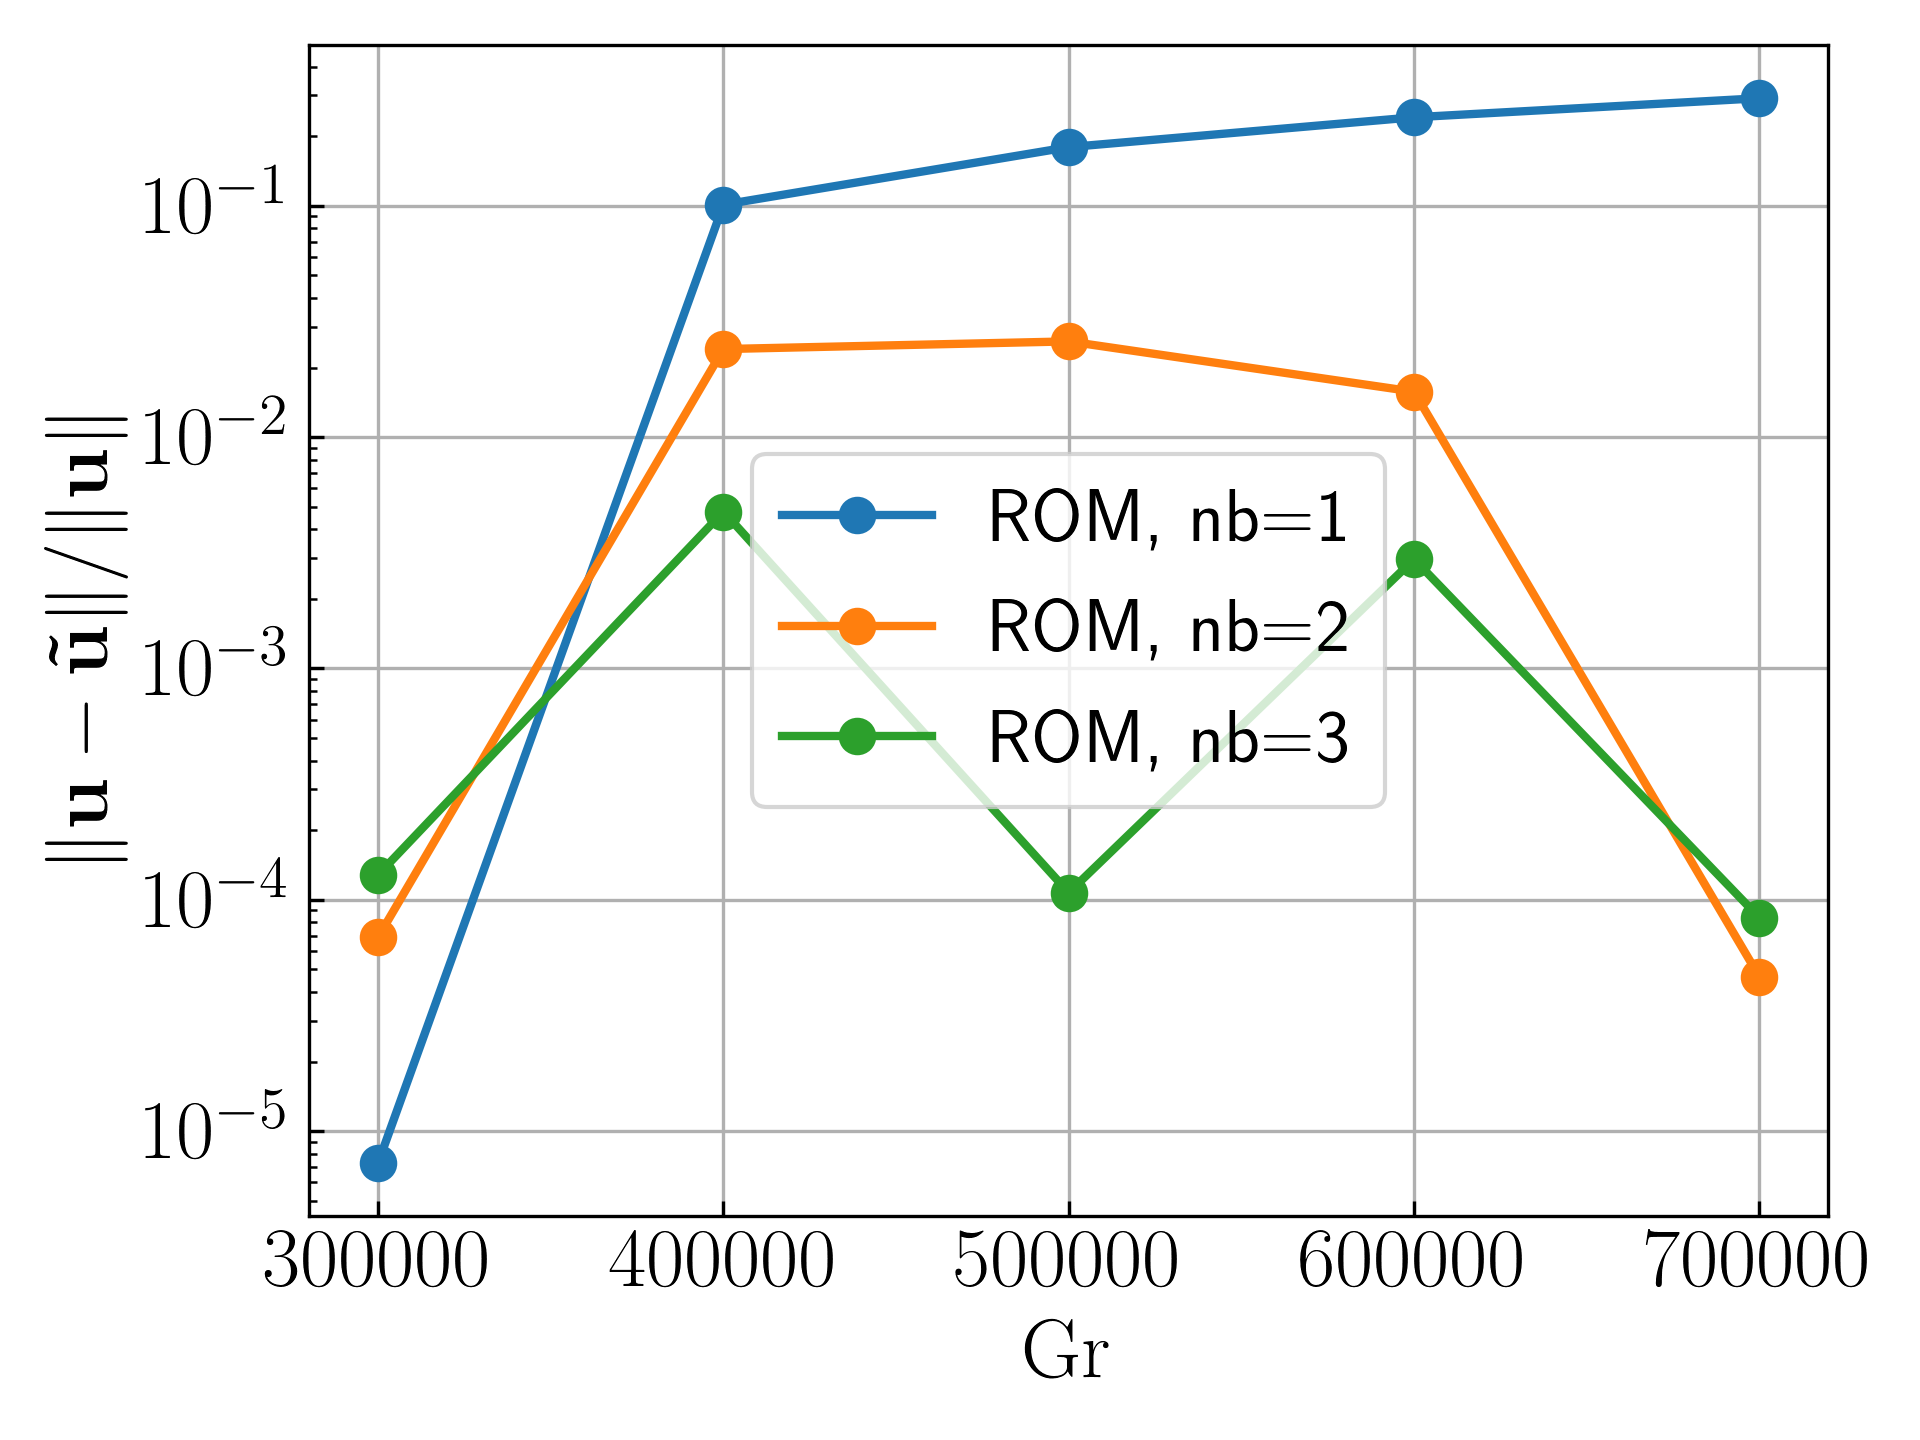
\includegraphics[width=\textwidth]{/Users/bigticket0501/NekMOR_cases/annulus_2d/pmor/err_gr}
         \caption{}
         \label{fig:3_a}
     \end{subfigure}
     \hfill
     \begin{subfigure}[b]{0.45\textwidth}
         \centering
         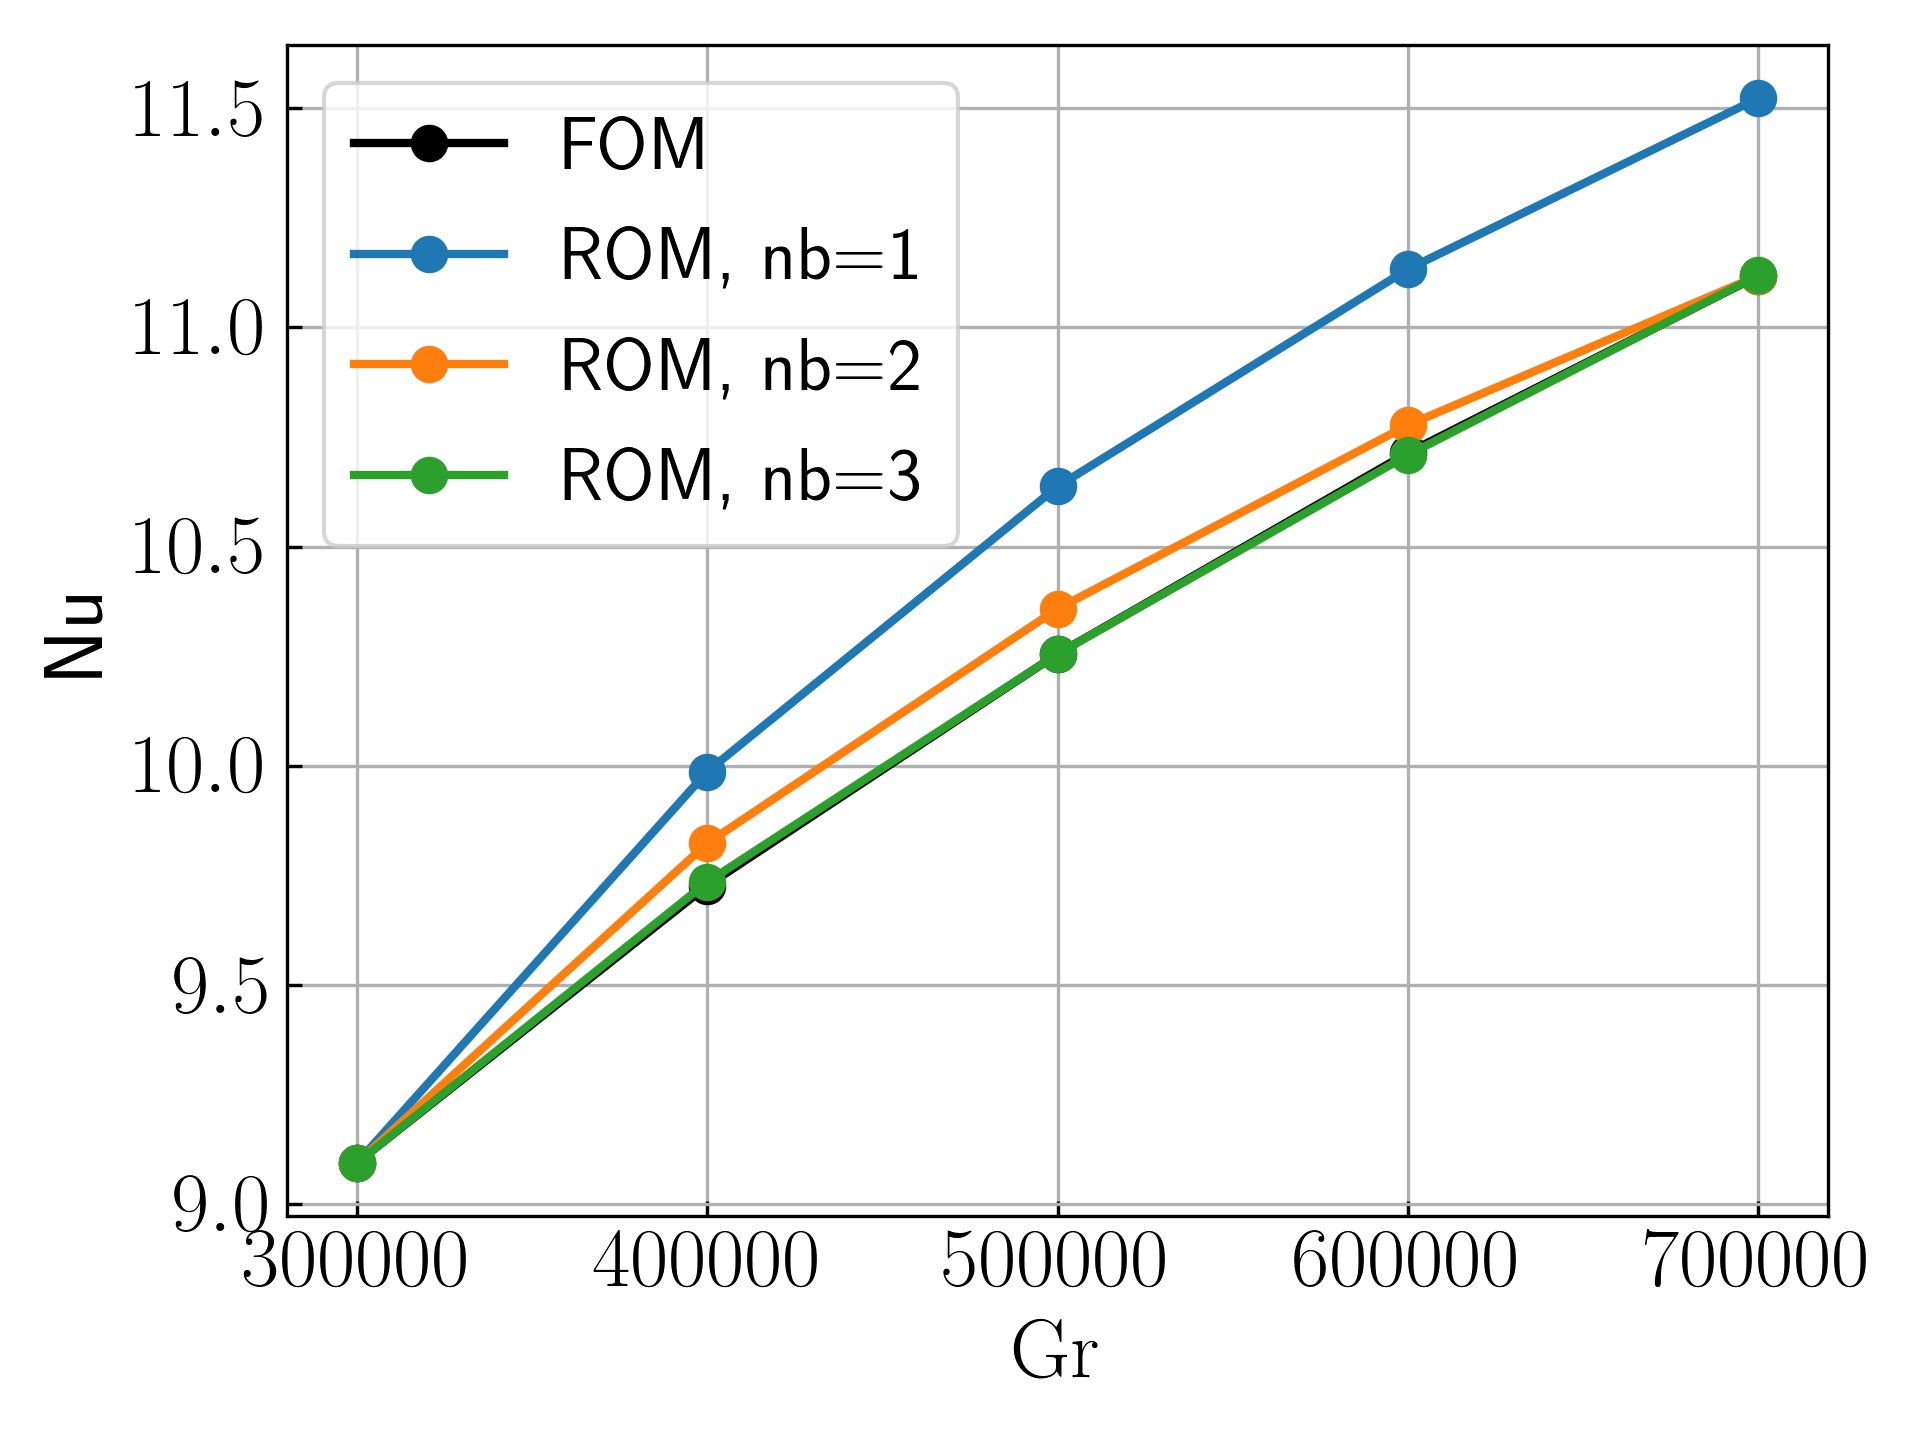
\includegraphics[width=\textwidth]{/Users/bigticket0501/NekMOR_cases/annulus_2d/pmor/nu_gr}
         \caption{}
         \label{fig:3_b}
     \end{subfigure}
     \caption{\subref{fig:3_a}: Relative $H^1$ error in the predicted solution
     with $N=1,~2,~3$.  \subref{fig:3_b}: Relative error in the predicted Nu
     with $N=1,~2,~3$; the ROM prediction values with $N=3$ are overlapped with
     the FOM values.} \label{fig:3}
\end{figure}

\newpage
\subsection{Heat Conduction Problem}
We consider a steady heat conduction problem in a two-dimensional domain
$\Omega = (-1,~1)\times(-1,~1)$. 
The strong formulation of this parametrized problem is stated as: for some
parameter value $\mu \in \mathbb{P}$, find $T(\mu)$ such that
%
\begin{equation*}
   \left\{
\begin{array}{llll}
   \nabla \cdot \kappa_\mu \nabla T(\mu) & = & 0 \quad & \text{in } \Omega\\
    \nabla T(\mu)                        & = & 0 \quad & \text{on } \Gamma_{top}\\
    \kappa_\mu \nabla T(\mu) \cdot n     & = & 0 \quad & \text{on } \Gamma_{side}\\
    \kappa_\mu \nabla T(\mu) \cdot n     & = & \mu_2 \quad & \text{on } \Gamma_{base}
\end{array}
\right.
\end{equation*}
%
where $\Gamma_{base} = (-1, 1)\times \{-1\}$, $\Gamma_{top} = (-1, 1)\times
\{1\}$, and $\Gamma_{side} = \{\pm 1\} \times (-1, 1)$.
Let $\Omega_0$ be a disk centered at the origin of radius $r_0=0.5$ and define
$\Omega_1 = \Omega \slash \overline{\Omega}_0$. The conductivity $\kappa_\mu =
\mathbbm{1}_{\Omega_1} + \mu_1 \mathbbm{1}_{\Omega_0}$. We consider $P=2$
parameters and $\mathbb{P} = [ \mu^{min}_1, \mu^{max}_1] \times [\mu^{min}_2,
\mu^{max}_2]$. The parameter vector is thus given by $\mu= (\mu_1, \mu_2)$.

The output of interest is the average temperature over $\Gamma_{base}$,
%
\begin{equation}
   s(\mu) = \ell(T(\mu);\mu) = \mu_2 \int_{\Gamma_{base}} T(\mu).
\end{equation}
%
The weak parametrized formulation reads: for
some parameter $\mu \in \mathbb{P}$, find $T(\mu) \in \mathbb{V}$ such that
%
\begin{align}
   a(T(\mu), v; \mu) = f(v;\mu)\quad \forall v \in \mathbb{V},
\end{align}
%
with
\begin{equation}
   a(w, v; \mu) = \int_{\Omega} \kappa_\mu \nabla w \cdot \nabla
   v \quad \text{and} \quad f(v; \mu) = \mu_2 \int_{\Gamma_{base}} v,
\end{equation} for all $v,~w \in \mathbb{V}$.

In Fig.~\ref{fig:hc_fom}, four representative solutions are shown with different
values of the parameters.
\begin{figure}[!h]
     \centering
     \begin{subfigure}[b]{0.45\textwidth}
         \centering
         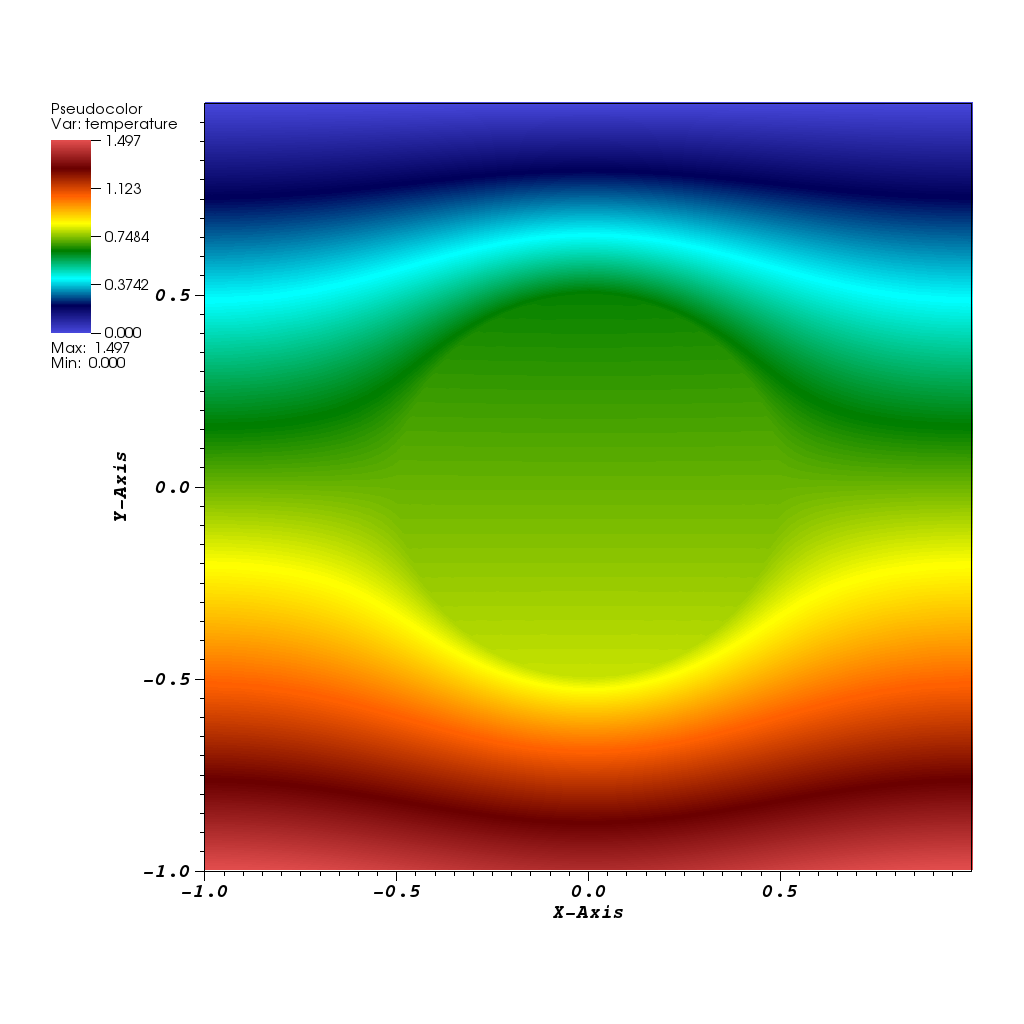
\includegraphics[width=\textwidth]{visit0039}
         \caption{$\mu= (10, 1)$}
     \end{subfigure}
     \hfill
     \begin{subfigure}[b]{0.45\textwidth}
         \centering
         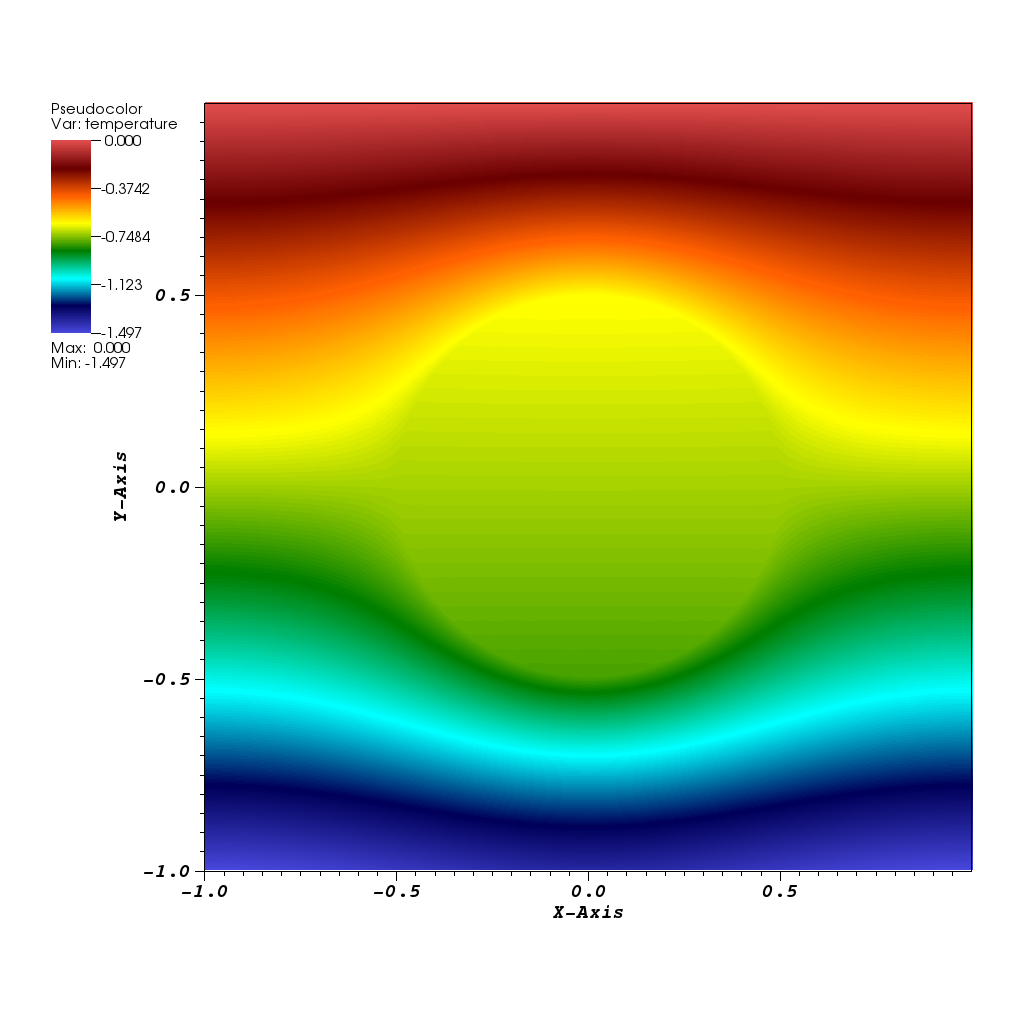
\includegraphics[width=\textwidth]{visit0040}
         \caption{$\mu = (10, -1)$}
     \end{subfigure}\\
     \begin{subfigure}[b]{0.45\textwidth}
         \centering
         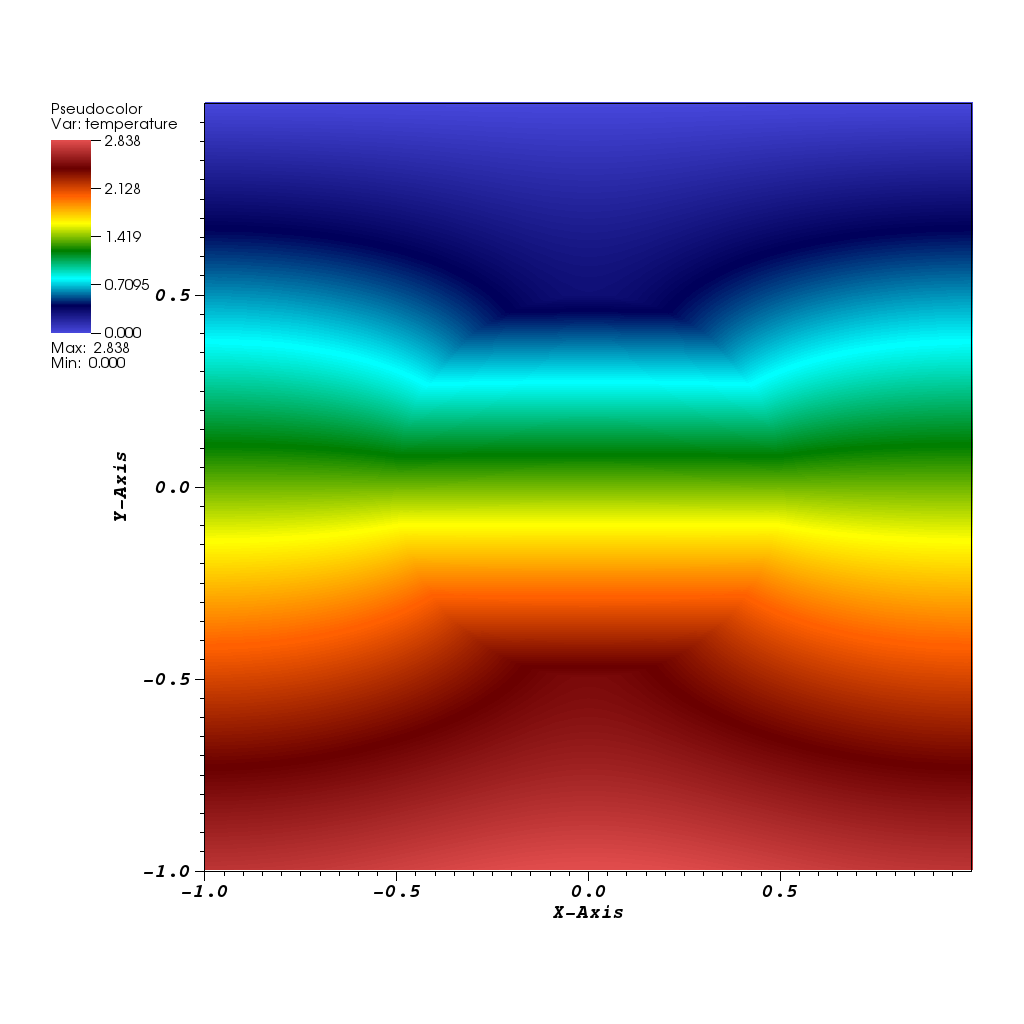
\includegraphics[width=\textwidth]{visit0041}
         \caption{$\mu = (0.1, 1)$}
     \end{subfigure}
     \hfill
     \begin{subfigure}[b]{0.45\textwidth}
         \centering
         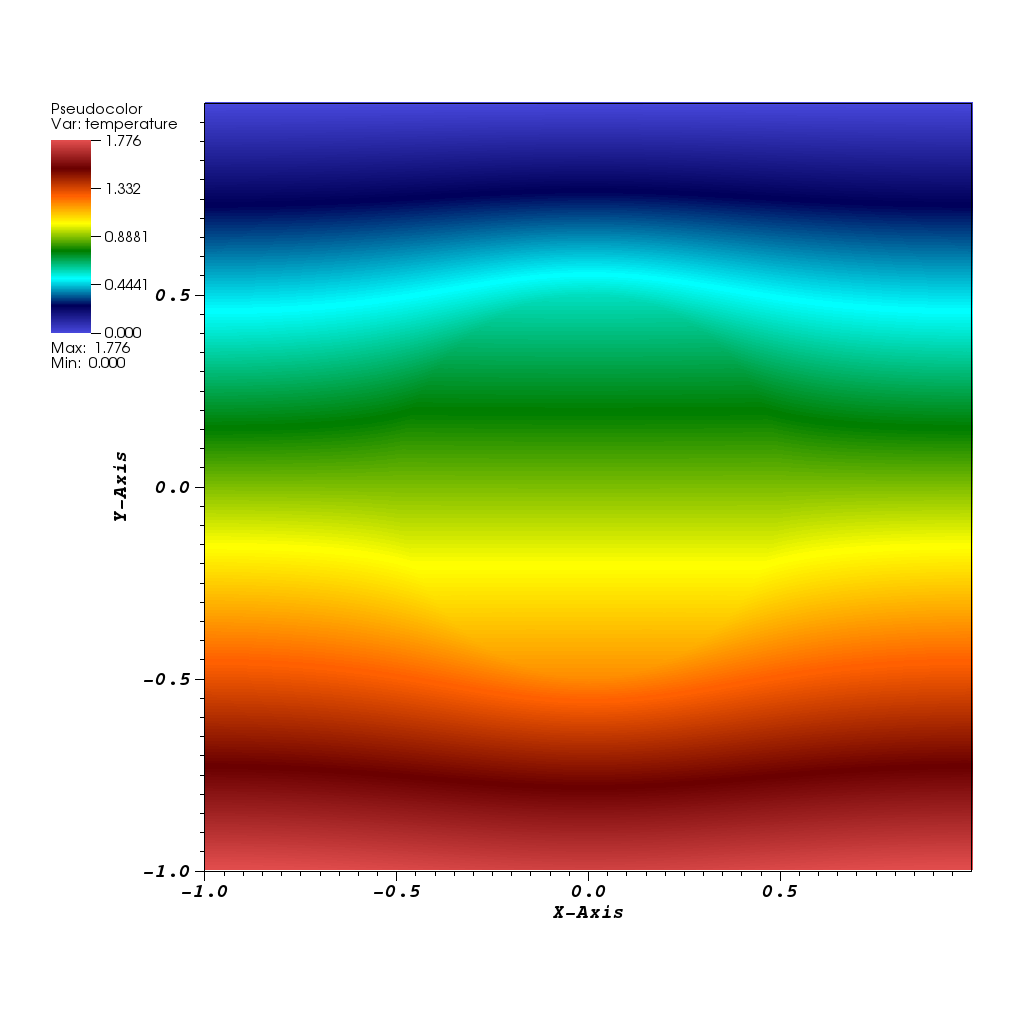
\includegraphics[width=\textwidth]{visit0042}
         \caption{$\mu = (2, 1)$}
     \end{subfigure}
     \caption{FOM solutions at different $\mu = (\mu_1,\mu_2)$, where $\mu_1$
     is the conductivity in the disk and $\mu_2$ is the heat flux over
     $\Gamma_{base}$.}
      \label{fig:hc_fom}
\end{figure}

\begin{figure}[!h]
     \centering
     \begin{subfigure}[b]{0.5\textwidth}
         \centering
         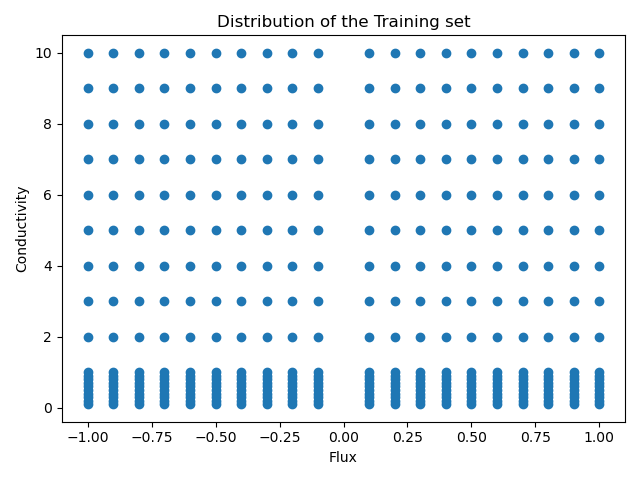
\includegraphics[width=\textwidth]{train_set_1}
         \caption{$380$ training data, where $(\kappa, flux) \in [0.1,~10] \times [-1, 1]$}
         \label{fig:6_a}
     \end{subfigure}\\
     \begin{subfigure}[b]{0.45\textwidth}
         \centering
         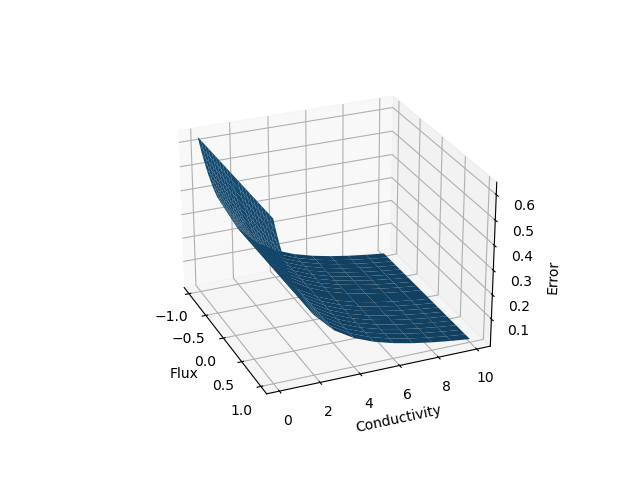
\includegraphics[width=\textwidth]{err_surf_1}
         \caption{Relative error with one anchor point $(10, 1)$}
         \label{fig:6_b}
     \end{subfigure}
     \hfill
     \begin{subfigure}[b]{0.45\textwidth}
         \centering
         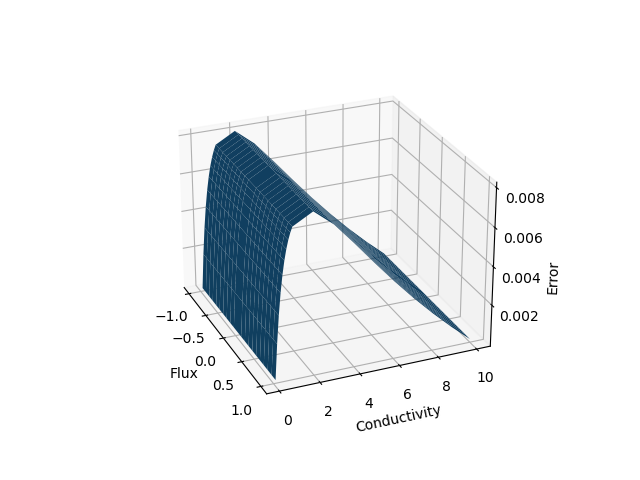
\includegraphics[width=\textwidth]{err_surf_2}
         \caption{Relative error with two anchor points $(10, 1)$ and $(0.1, 1)$}
         \label{fig:6_c}
     \end{subfigure}
     \caption{}
      \label{fig:6}
\end{figure}

\begin{figure}[!h]
     \centering
     \begin{subfigure}[b]{0.45\textwidth}
         \centering
         \includegraphics[width=\textwidth]{/Users/bigticket0501/NekMOR_cases/poisson/param_cond_heatf/rom/coer_compare}
     \end{subfigure}
     \caption{FOM coercivity constant with different intrinsic norm
     $\|\cdot\|_{\mathbb{V}}$. Coercivity constant $\alpha(\mu) \coloneqq
     \inf_{v} \frac{a(v,v;\mu)}{\|v\|^2_{\mathbb{V}}}$}
\end{figure}

\begin{figure}[!h]
     \centering
     \begin{subfigure}[b]{0.45\textwidth}
         \centering
         \includegraphics[width=\textwidth]{/Users/bigticket0501/NekMOR_cases/poisson/param_cond_heatf/rom/coer_coerlb}
     \end{subfigure}
     \caption{Estimated lower bound for the coercivity constant using Min-$\theta$ approach.}
\end{figure}

\begin{figure}[!h]
     \centering
     \begin{subfigure}[b]{0.45\textwidth}
         \centering
         \includegraphics[width=\textwidth]{/Users/bigticket0501/NekMOR_cases/poisson/param_cond_heatf/rom/ee_vs_solerr_cond0p1}
     \end{subfigure}
     \hfill
     \begin{subfigure}[b]{0.45\textwidth}
         \centering
         \includegraphics[width=\textwidth]{/Users/bigticket0501/NekMOR_cases/poisson/param_cond_heatf/rom/ee_vs_solerr_flux-1}
     \end{subfigure}
\end{figure}

\begin{figure}[!h]
     \centering
     \begin{subfigure}[b]{0.45\textwidth}
         \centering
         \includegraphics[width=\textwidth]{/Users/bigticket0501/NekMOR_cases/poisson/param_cond_heatf/rom/ee_vs_qoierr_cond0p1}
     \end{subfigure}
     \hfill
     \begin{subfigure}[b]{0.45\textwidth}
         \centering
         \includegraphics[width=\textwidth]{/Users/bigticket0501/NekMOR_cases/poisson/param_cond_heatf/rom/ee_vs_qoierr_flux-1}
     \end{subfigure}
\end{figure}

\newpage
\subsection{Kovasznay Solution}
Kovasznay gives an analytical solution to the steady-state Navier-Stokes
equations that is similar to the two-dimensional flow-field behind a periodic
array of cylinders,
\begin{align}
   u_x = 1-e^{\lambda x} \cos(2 \pi y), \quad u_y = \frac{\lambda}{2\pi}
   e^{\lambda x} \sin(2 \pi y),
\end{align}
where $\lambda \coloneqq \rm Re/2 - \sqrt{\rm Re^2/4 + 4\pi^2}$. 

In this model problem, the parameter $\rm Re$ also appears in the boundary
condition, therefore, in order to apply pMOR, we consider the Galerkin ROM with
penalty methods. The coarse system is modified as:
\begin{equation} \label{eq:rom}
     H_{\tc,\nu}  \,{\huu_\tc}^n  = \bB^T \, {\hat \buf}(\bbu_\tc^n,\bT_\tc^n;
     \theta_g) + \tau ( \sum^{N_{BC}}_{k=1}( U_{BC,k} D^k - E^k{\huu_\tc}^n )).
\end{equation}
The additional boundary terms are defined as:
\begin{equation}
   (D^k)_i = (\bzeta_i)_{L^2(\Gamma_{D_k})},\quad (E^k)_{ij} = (\bzeta_i,
   \bzeta_j)_{L^2(\Gamma_{D_k})}.
\end{equation}


\begin{figure}[!h]
     \centering
     \begin{subfigure}[b]{0.45\textwidth}
         \centering
         \includegraphics[width=\textwidth]{/Users/bigticket0501/NekExamples/kovasznay/Re40/visit0002}
         \caption{$\rm Re=40$}
         \label{fig:4_a}
     \end{subfigure}
     \hfill
     \begin{subfigure}[b]{0.45\textwidth}
         \centering
         \includegraphics[width=\textwidth]{/Users/bigticket0501/NekExamples/kovasznay/Re60/visit0001}
         \caption{$\rm Re=60$}
         \label{fig:4_b}
     \end{subfigure}\\
     \begin{subfigure}[b]{0.45\textwidth}
         \centering
         \includegraphics[width=\textwidth]{/Users/bigticket0501/NekExamples/kovasznay/Re80/visit0003}
         \caption{$\rm Re=80$}
         \label{fig:4_c}
     \end{subfigure}
     \hfill
     \begin{subfigure}[b]{0.45\textwidth}
         \centering
         \includegraphics[width=\textwidth]{/Users/bigticket0501/NekExamples/kovasznay/Re100/visit0005}
         \caption{$\rm Re=100$}
         \label{fig:4_d}
     \end{subfigure}
     \caption{\subref{fig:4_a}--\subref{fig:4_d}: FOM solution at $\rm
     Re=40,~60,~80,~100$.} \label{fig:4}
\end{figure}

\newpage
\subsection{Flow pass a cylinder}
\subsubsection{Application of penalty methods - parametrized inlet velocity}
\begin{figure}[!h]
     \centering
     \begin{subfigure}[b]{0.45\textwidth}
         \centering
         \includegraphics[width=\textwidth]{cyl_Re100_u1}
         \caption{$\rm Re=100$, with $u=1$}
         \label{fig:5_a}
     \end{subfigure}
     \hfill
     \begin{subfigure}[b]{0.45\textwidth}
         \centering
         \includegraphics[width=\textwidth]{cyl_Re100_u2}
         \caption{$\rm Re=100$, with $u=2$}
         \label{fig:5_b}
     \end{subfigure}\\
     \begin{subfigure}[b]{0.45\textwidth}
         \centering
         \includegraphics[width=\textwidth]{cyl_Re100_u3}
         \caption{$\rm Re=100$, with $u=3$}
         \label{fig:5_c}
     \end{subfigure}
     \caption{\subref{fig:5_a}--\subref{fig:5_c}: Snapshots at $\rm
     Re=100$ with $u=1,~2,~3$..} \label{fig:5}
\end{figure}

\subsubsection{One anchor point $(\rm Re, u_{inlet}) = (100, 1)$}
\begin{figure}[!h]
     \centering
     \begin{subfigure}[b]{0.3\textwidth}
         \centering
         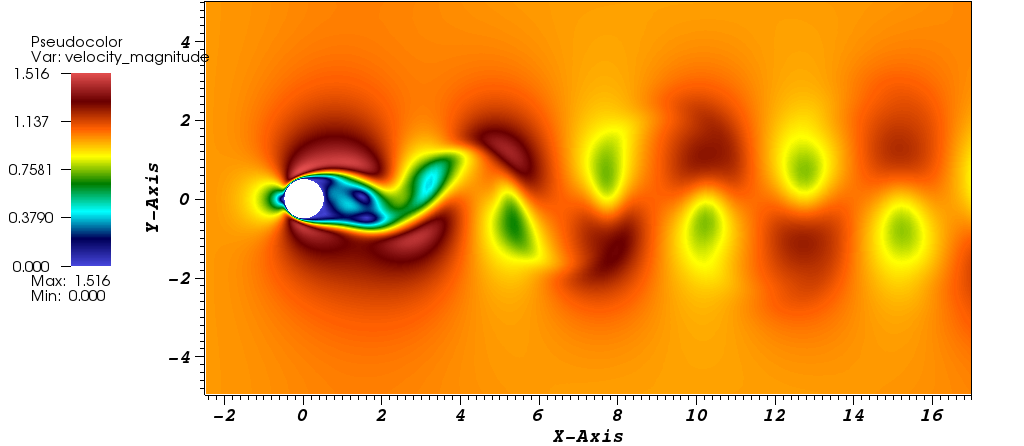
\includegraphics[width=\textwidth]{anchor_1/visit0009}
         \caption{ROM, $u=1$}
         \label{fig:6_a}
     \end{subfigure}
     \hfill
     \begin{subfigure}[b]{0.3\textwidth}
         \centering
         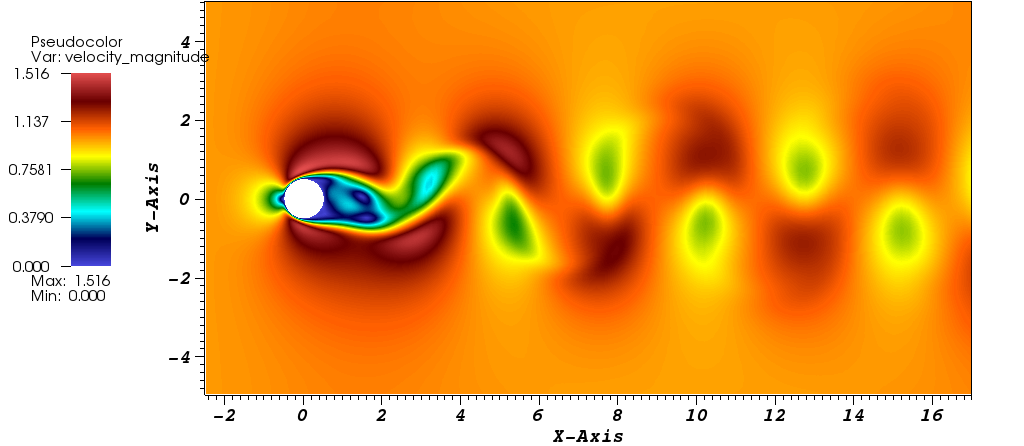
\includegraphics[width=\textwidth]{anchor_1/visit0010}
         \caption{FOM, $u=1$}
         \label{fig:6_b}
     \end{subfigure}
     \hfill
     \begin{subfigure}[b]{0.3\textwidth}
         \centering
         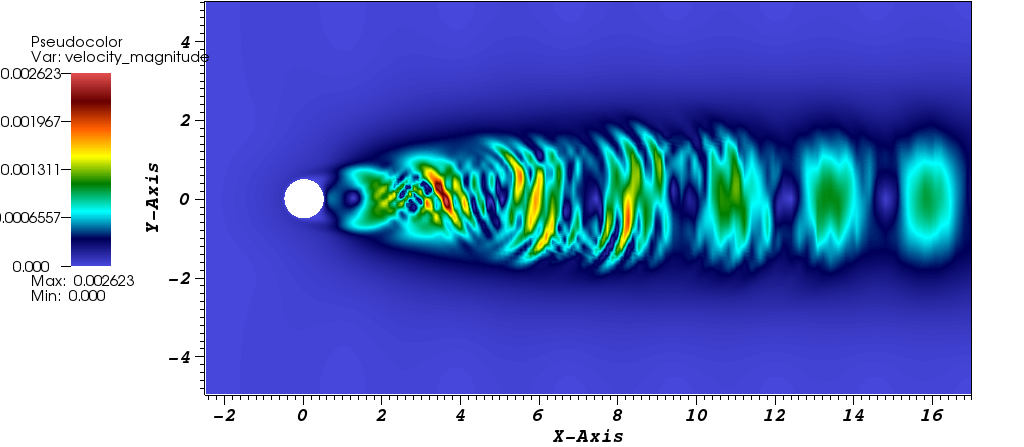
\includegraphics[width=\textwidth]{anchor_1/visit0011}
         \caption{Difference, $u=1$}
         \label{fig:6_c}
     \end{subfigure}\\
     \begin{subfigure}[b]{0.3\textwidth}
         \centering
         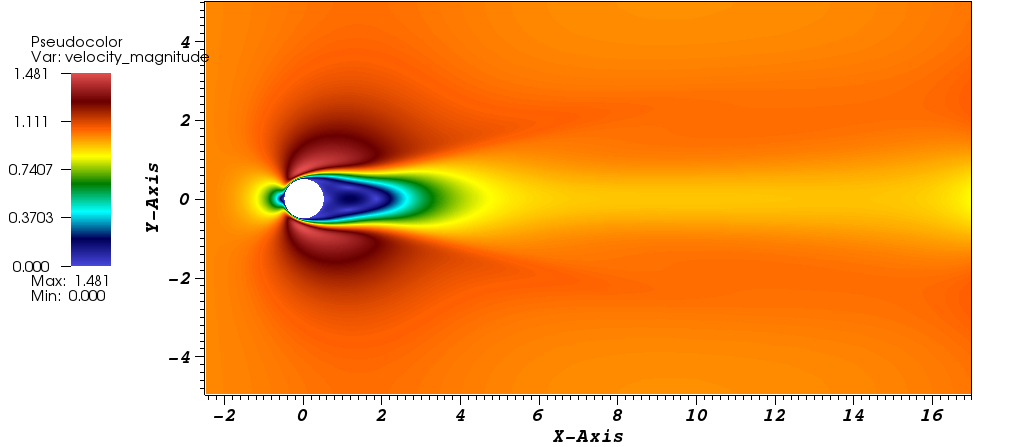
\includegraphics[width=\textwidth]{anchor_1/visit0012}
         \caption{ROM, $u=1$}
         \label{fig:6_d}
     \end{subfigure}
     \hfill
     \begin{subfigure}[b]{0.3\textwidth}
         \centering
         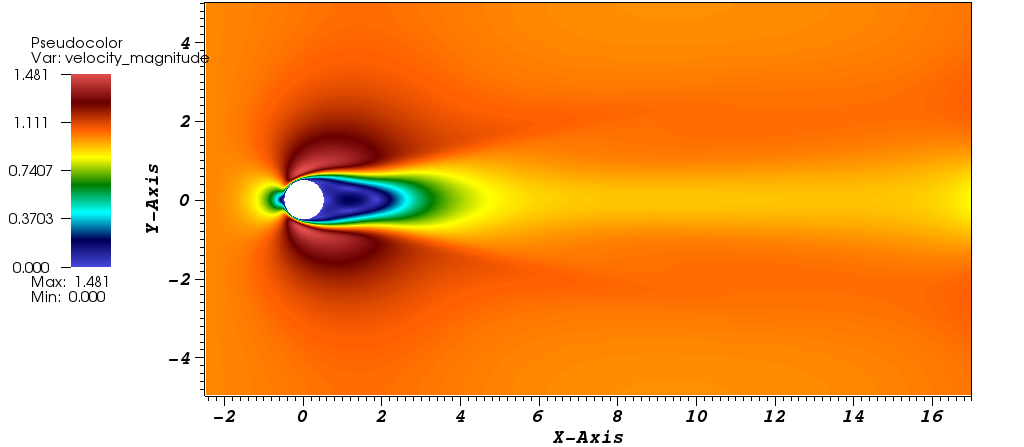
\includegraphics[width=\textwidth]{anchor_1/visit0013}
         \caption{FOM, $u=1$}
         \label{fig:6_e}
     \end{subfigure}
     \hfill
     \begin{subfigure}[b]{0.3\textwidth}
         \centering
         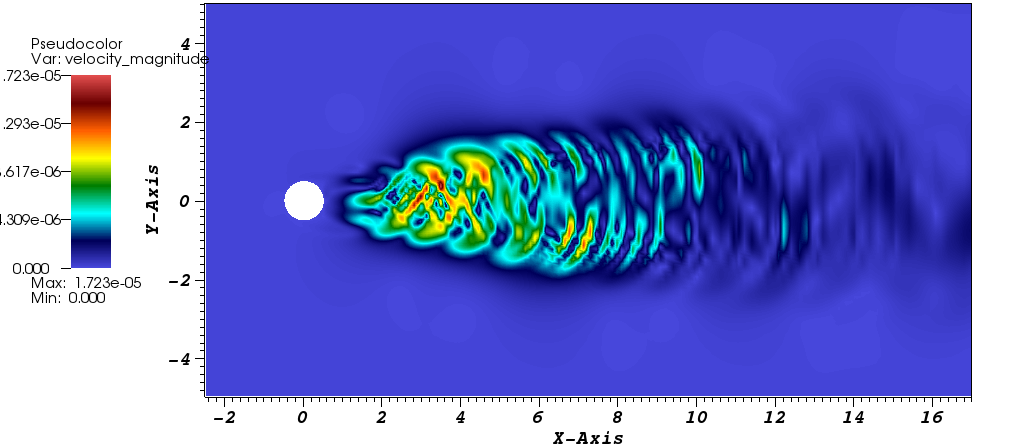
\includegraphics[width=\textwidth]{anchor_1/visit0014}
         \caption{Difference, $u=1$}
         \label{fig:6_f}
     \end{subfigure} 
     \caption{Performance with one anchor point.
     \subref{fig:6_a}--\subref{fig:6_c}: Solution comparison between ROM and
     FOM and its difference at $t=1000$. Maximum difference $\approx 3e-3$.
     \subref{fig:6_d}--\subref{fig:6_f}: Averaged solution comparison between
     ROM and FOM and its difference. Maximum difference $\approx 1.5e-5$.}
      \label{fig:6}
\end{figure}

\subsubsection{Two anchor points $(\rm Re, u_{inlet}) = (100, 1)$, $(\rm Re, u_{inlet}) = (100, 3)$}
\begin{figure}[h!]
     \centering
     \begin{subfigure}[b]{0.3\textwidth}
         \centering
         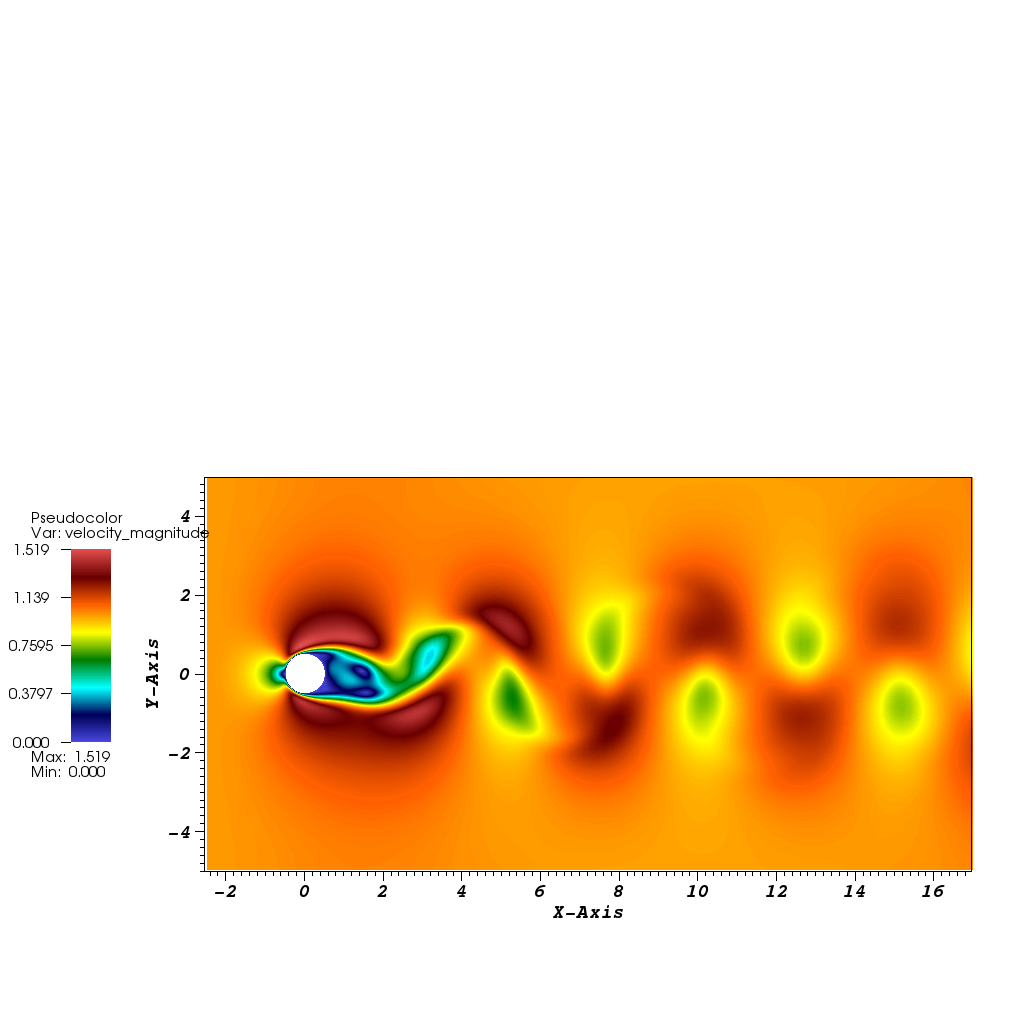
\includegraphics[width=\textwidth]{anchor_2/visit0022}
         \caption{ROM, $u=1$}
         \label{fig:6_a}
     \end{subfigure}
     \hfill
     \begin{subfigure}[b]{0.3\textwidth}
         \centering
         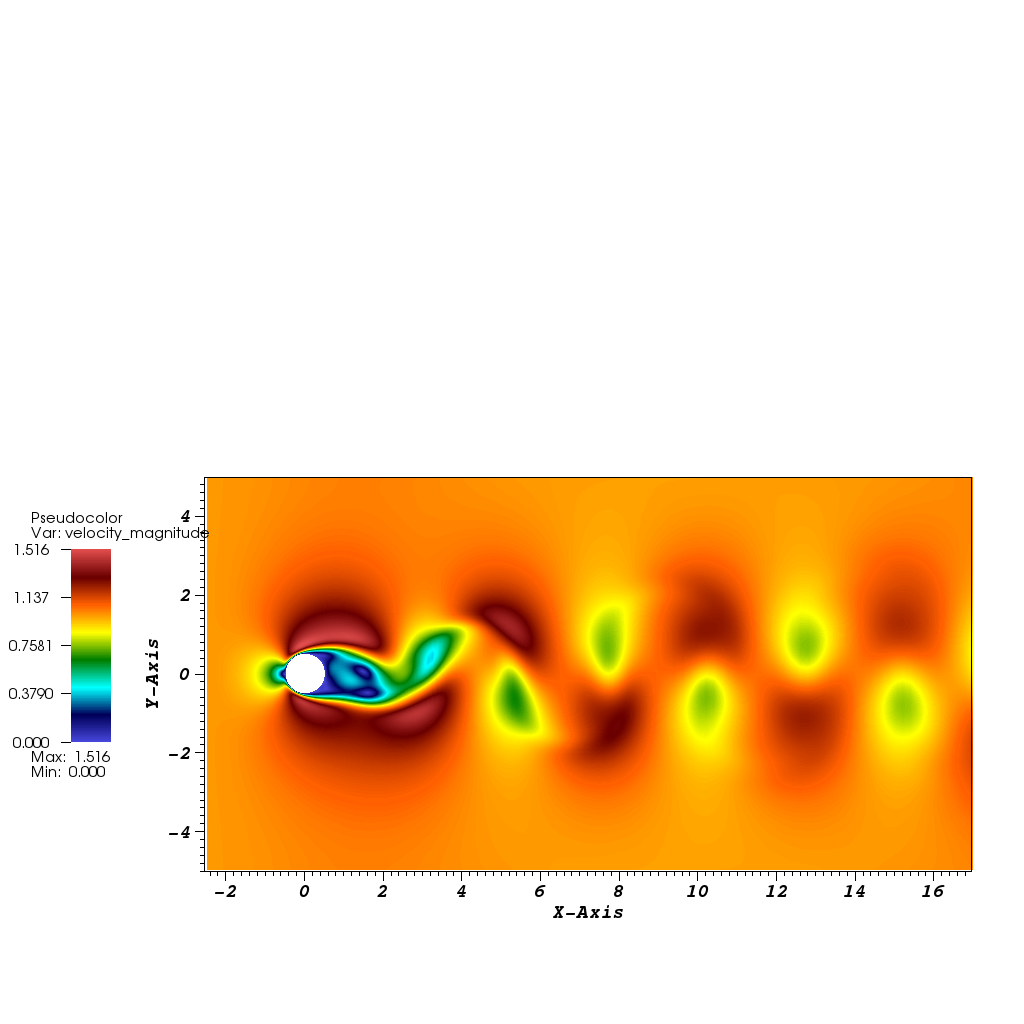
\includegraphics[width=\textwidth]{anchor_2/visit0023}
         \caption{FOM, $u=1$}
         \label{fig:6_b}
     \end{subfigure}
     \hfill
     \begin{subfigure}[b]{0.3\textwidth}
         \centering
         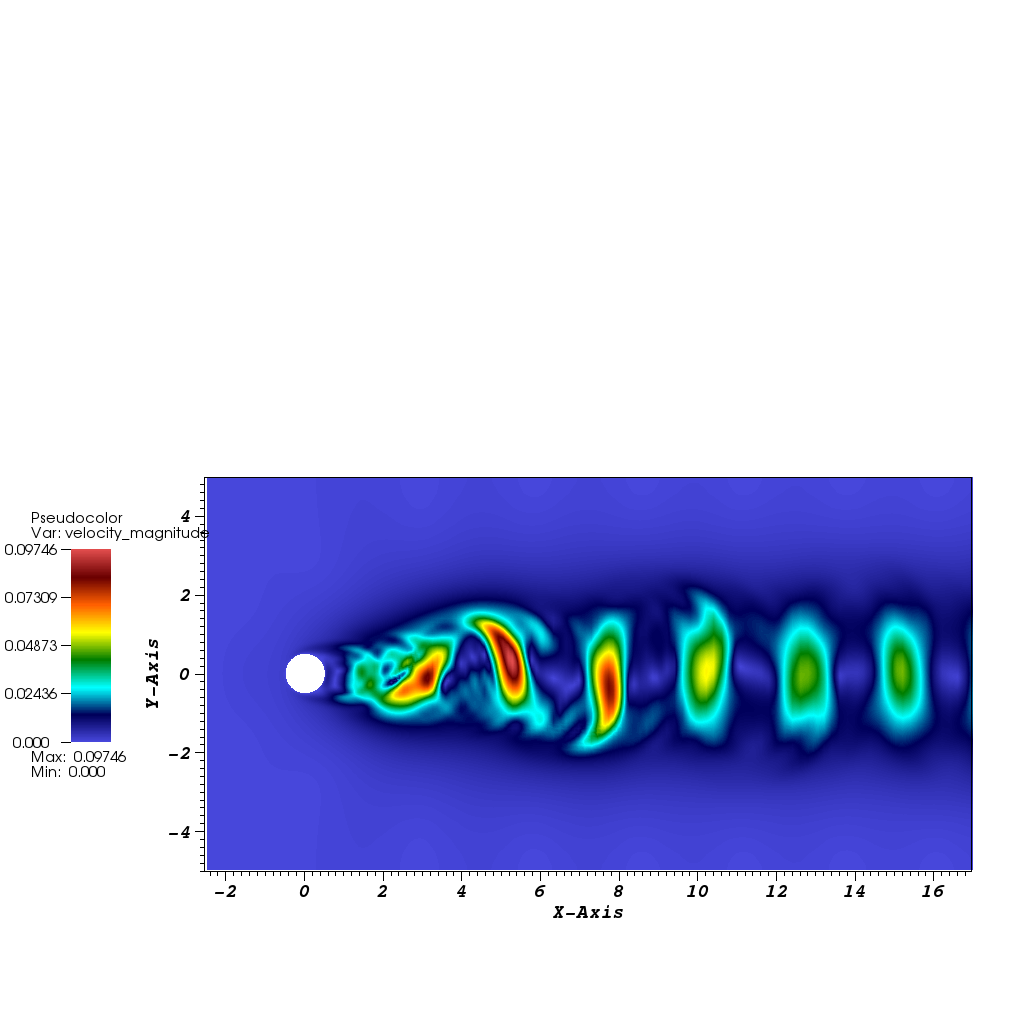
\includegraphics[width=\textwidth]{anchor_2/visit0024}
         \caption{Difference, $u=1$}
         \label{fig:6_c}
     \end{subfigure}\\
     \begin{subfigure}[b]{0.3\textwidth}
         \centering
         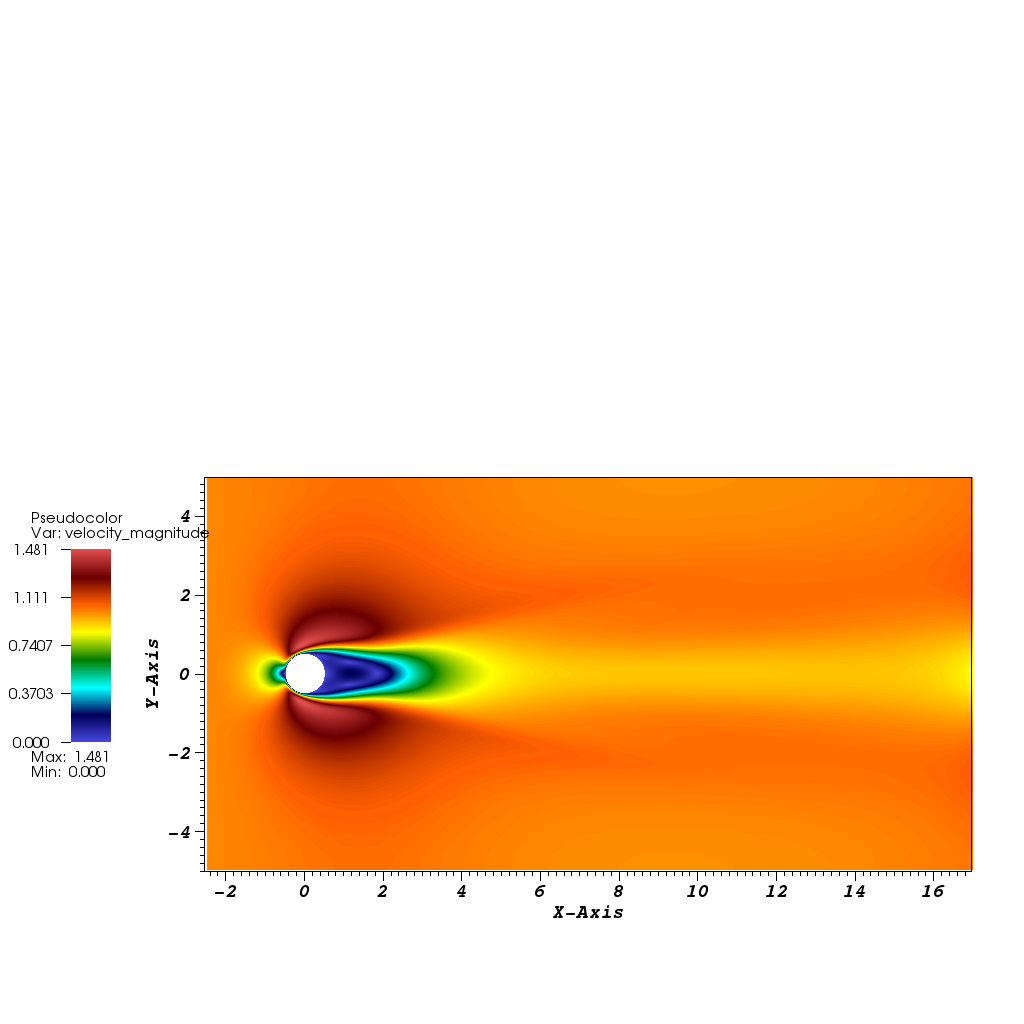
\includegraphics[width=\textwidth]{anchor_2/visit0025}
         \caption{ROM}, $u=1$
         \label{fig:6_d}
     \end{subfigure}
     \hfill
     \begin{subfigure}[b]{0.3\textwidth}
         \centering
         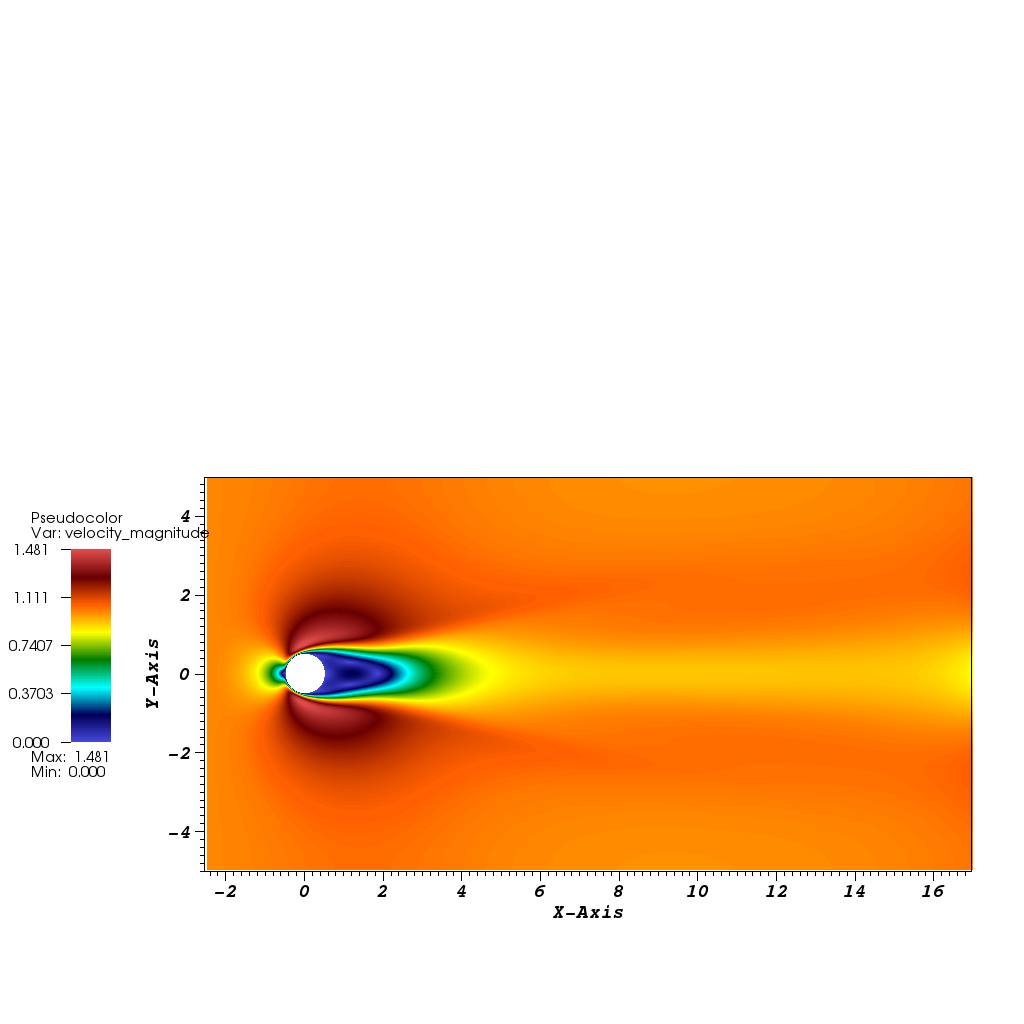
\includegraphics[width=\textwidth]{anchor_2/visit0026}
         \caption{FOM}, $u=1$
         \label{fig:6_e}
     \end{subfigure}
     \hfill
     \begin{subfigure}[b]{0.3\textwidth}
         \centering
         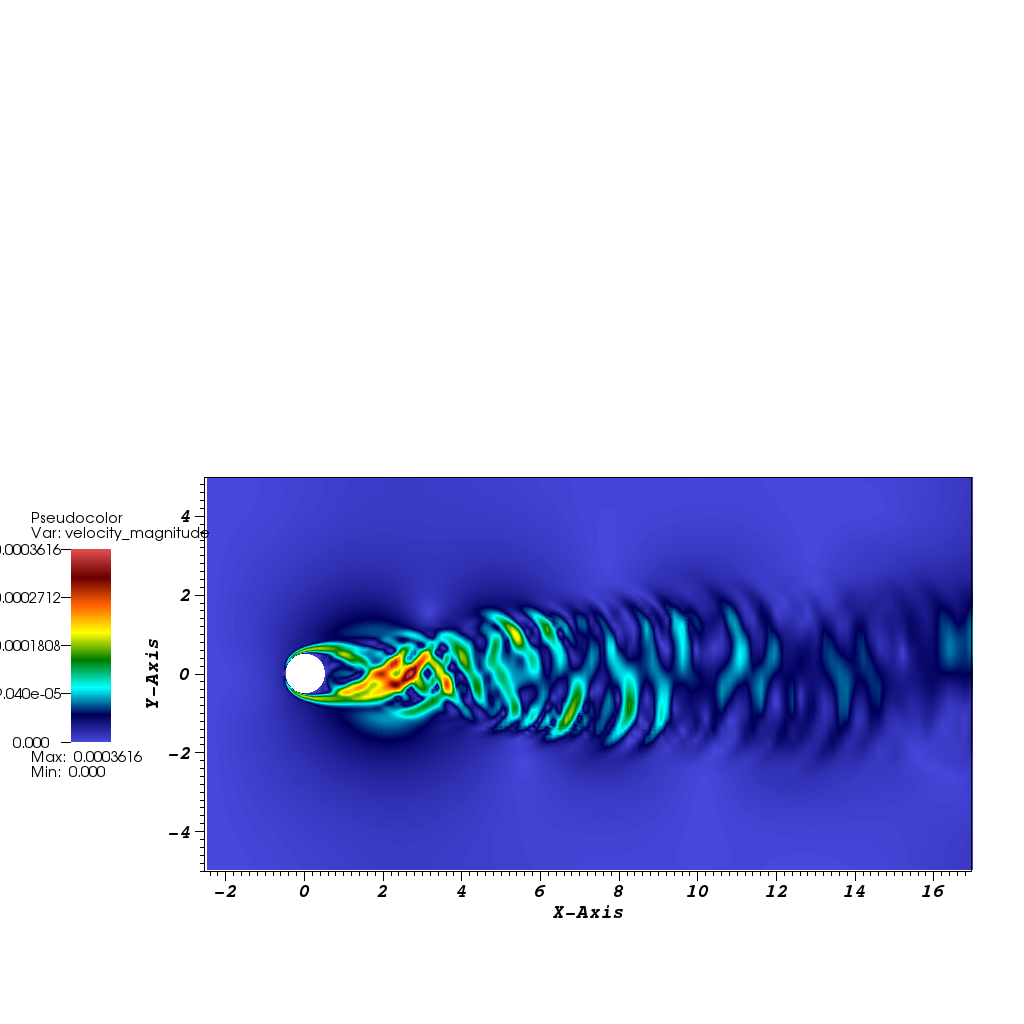
\includegraphics[width=\textwidth]{anchor_2/visit0027}
         \caption{Difference, $u=1$}
         \label{fig:6_f}
     \end{subfigure} 
     \caption{Performance with two anchor points. \subref{fig:6_a}--\subref{fig:6_c}: Solution
     comparison between ROM and FOM and its difference at $t=1000$. Maximum
     difference $\approx 3e-3$.  \subref{fig:6_d}--\subref{fig:6_f}: Averaged
     solution comparison between ROM and FOM and its difference. Maximum
     difference $\approx 1.5e-5$.}
      \label{fig:6}
\end{figure}
\begin{figure}[!h]
     \centering
     \begin{subfigure}[b]{0.3\textwidth}
         \centering
         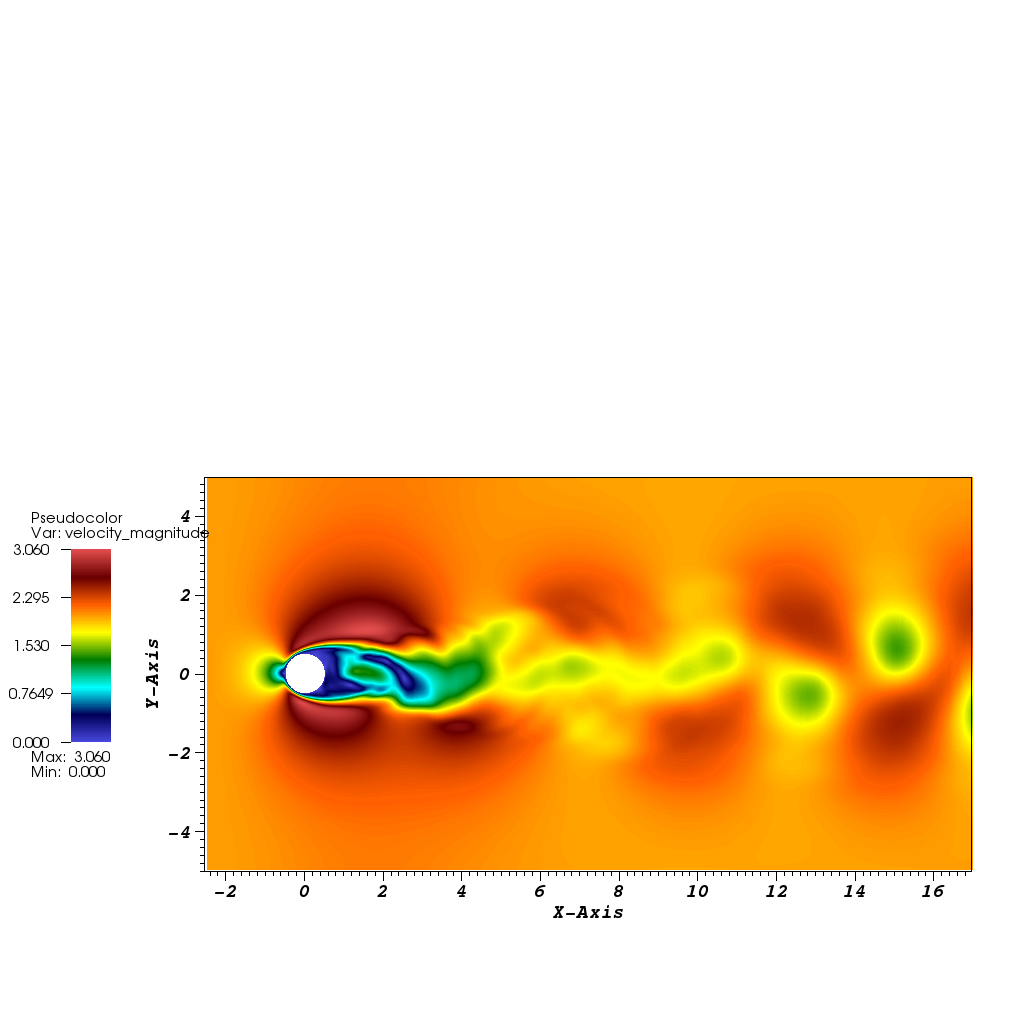
\includegraphics[width=\textwidth]{anchor_2/visit0028}
         \caption{ROM, $u=2$}
         \label{fig:6_a}
     \end{subfigure}
     \hfill
     \begin{subfigure}[b]{0.3\textwidth}
         \centering
         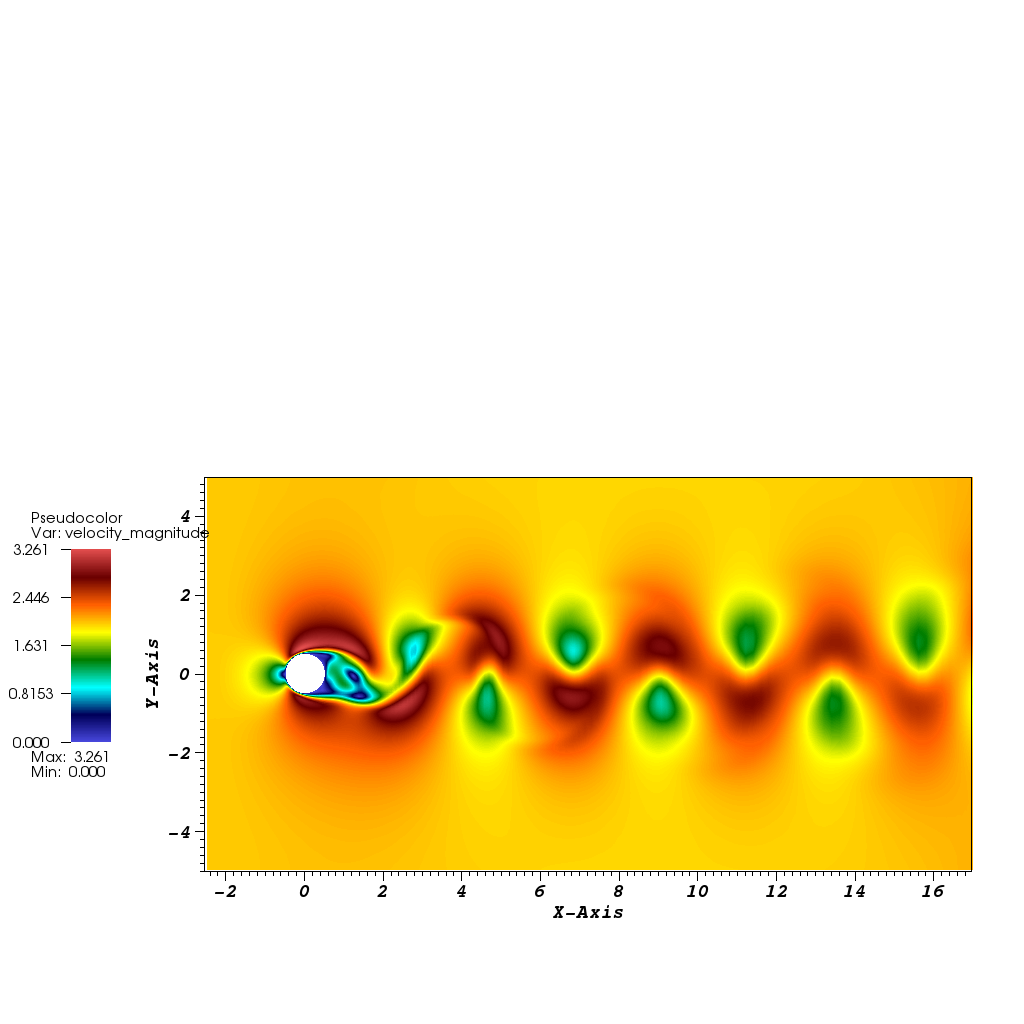
\includegraphics[width=\textwidth]{anchor_2/visit0029}
         \caption{FOM, $u=2$}
         \label{fig:6_b}
     \end{subfigure}
     \hfill
     \begin{subfigure}[b]{0.3\textwidth}
         \centering
         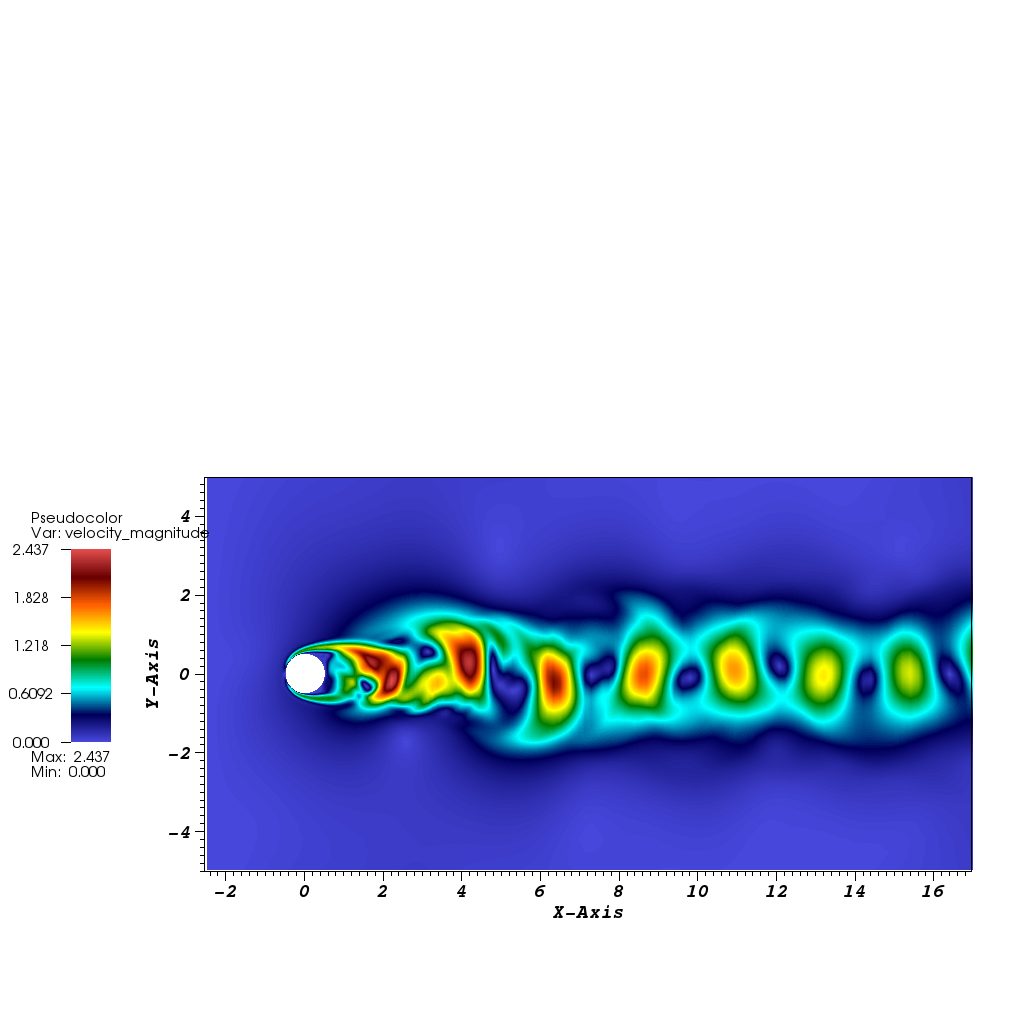
\includegraphics[width=\textwidth]{anchor_2/visit0030}
         \caption{Difference, $u=2$}
         \label{fig:6_c}
     \end{subfigure}\\
     \begin{subfigure}[b]{0.3\textwidth}
         \centering
         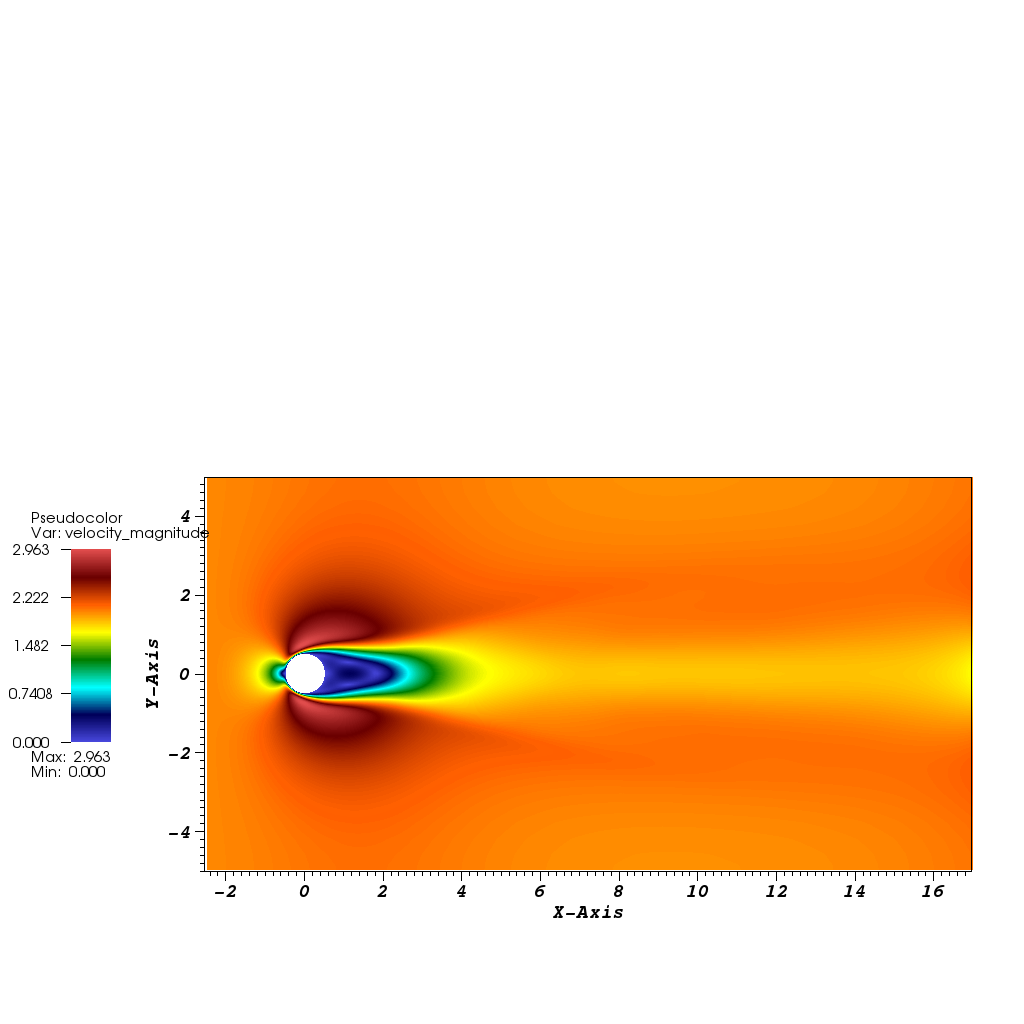
\includegraphics[width=\textwidth]{anchor_2/visit0031}
         \caption{ROM, $u=2$}
         \label{fig:6_d}
     \end{subfigure}
     \hfill
     \begin{subfigure}[b]{0.3\textwidth}
         \centering
         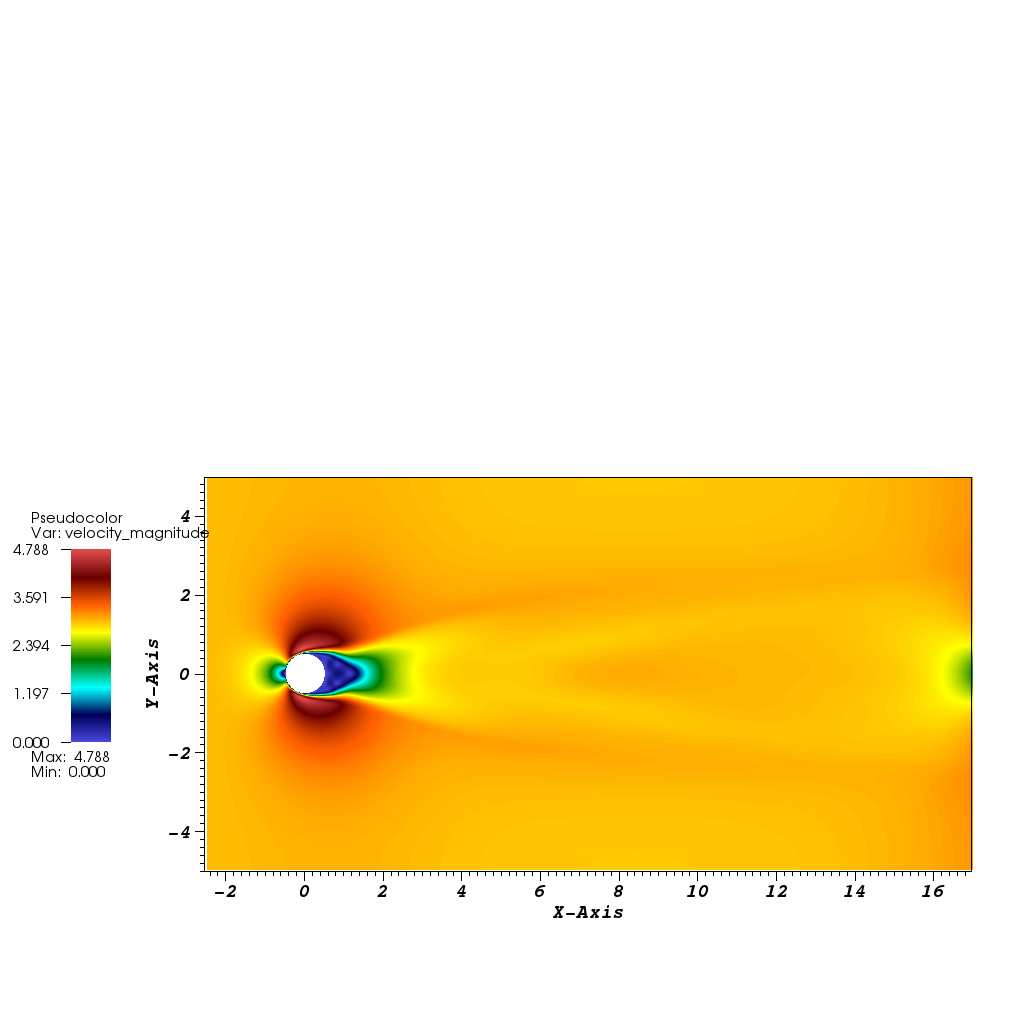
\includegraphics[width=\textwidth]{anchor_2/visit0032}
         \caption{FOM, $u=2$}
         \label{fig:6_e}
     \end{subfigure}
     \hfill
     \begin{subfigure}[b]{0.3\textwidth}
         \centering
         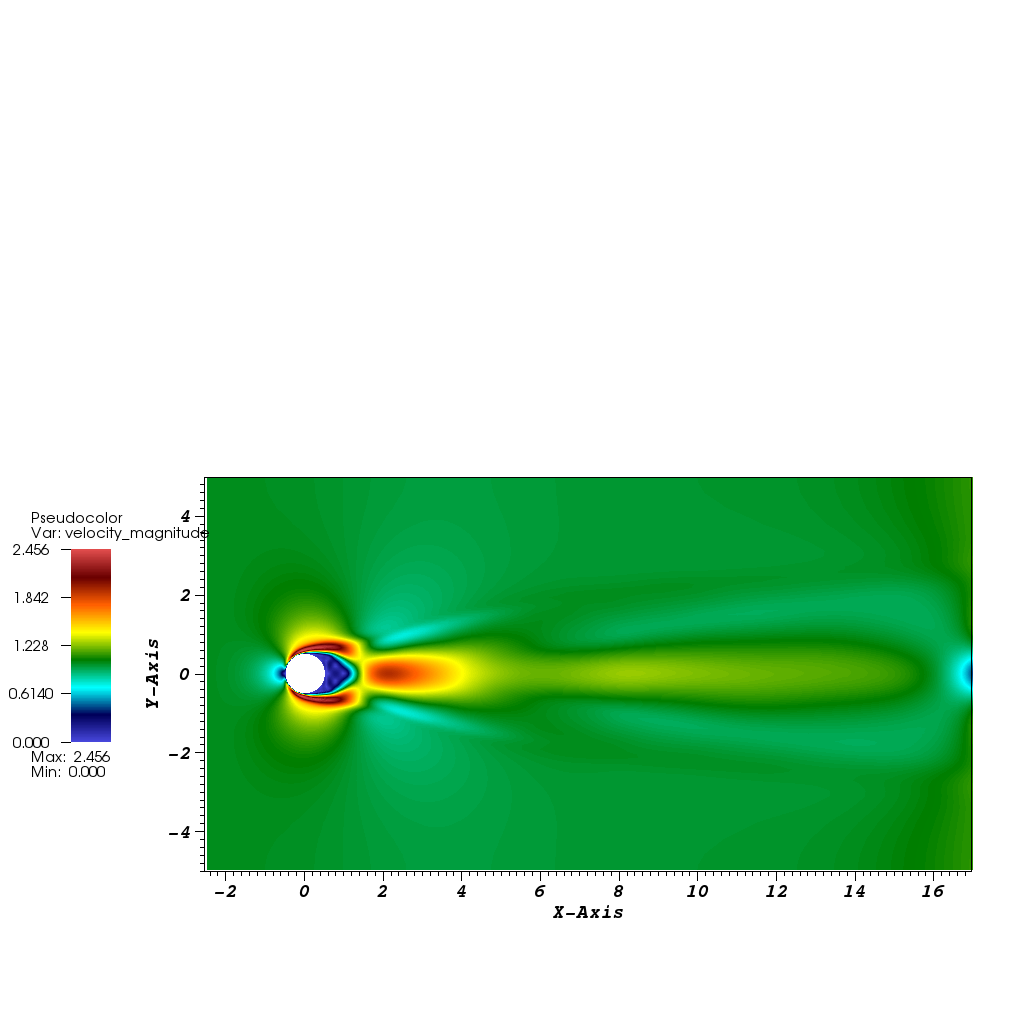
\includegraphics[width=\textwidth]{anchor_2/visit0033}
         \caption{Difference, $u=2$}
         \label{fig:6_f}
     \end{subfigure} 
     \caption{\subref{fig:6_a}--\subref{fig:6_c}: Solution comparison between
     ROM and FOM and its difference at $t=250$.
     \subref{fig:6_d}--\subref{fig:6_f}: Averaged solution comparison between
     ROM and FOM and its difference.}
      \label{fig:6}
\end{figure}
\begin{figure}[!h]
     \centering
     \begin{subfigure}[b]{0.3\textwidth}
         \centering
         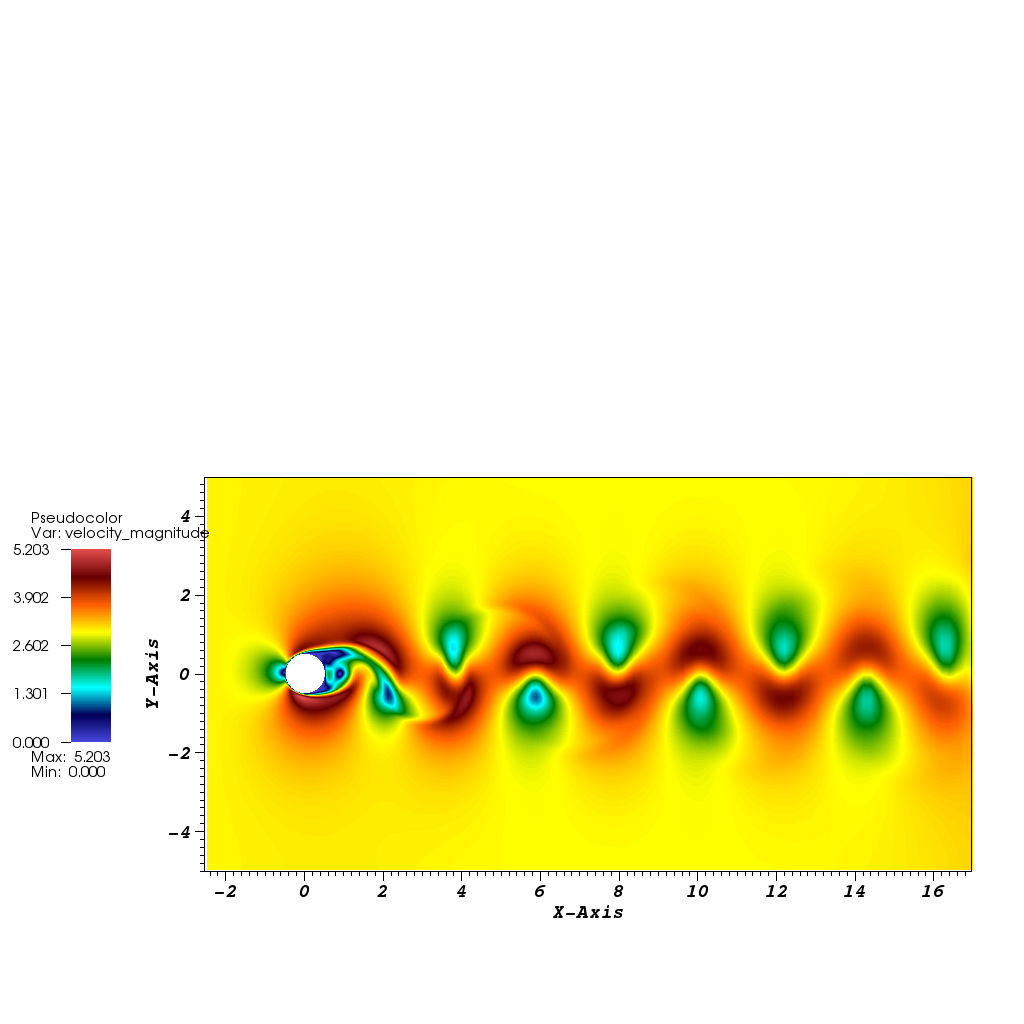
\includegraphics[width=\textwidth]{anchor_2/visit0015}
         \caption{ROM, $u=3$}
         \label{fig:6_a}
     \end{subfigure}
     \hfill
     \begin{subfigure}[b]{0.3\textwidth}
         \centering
         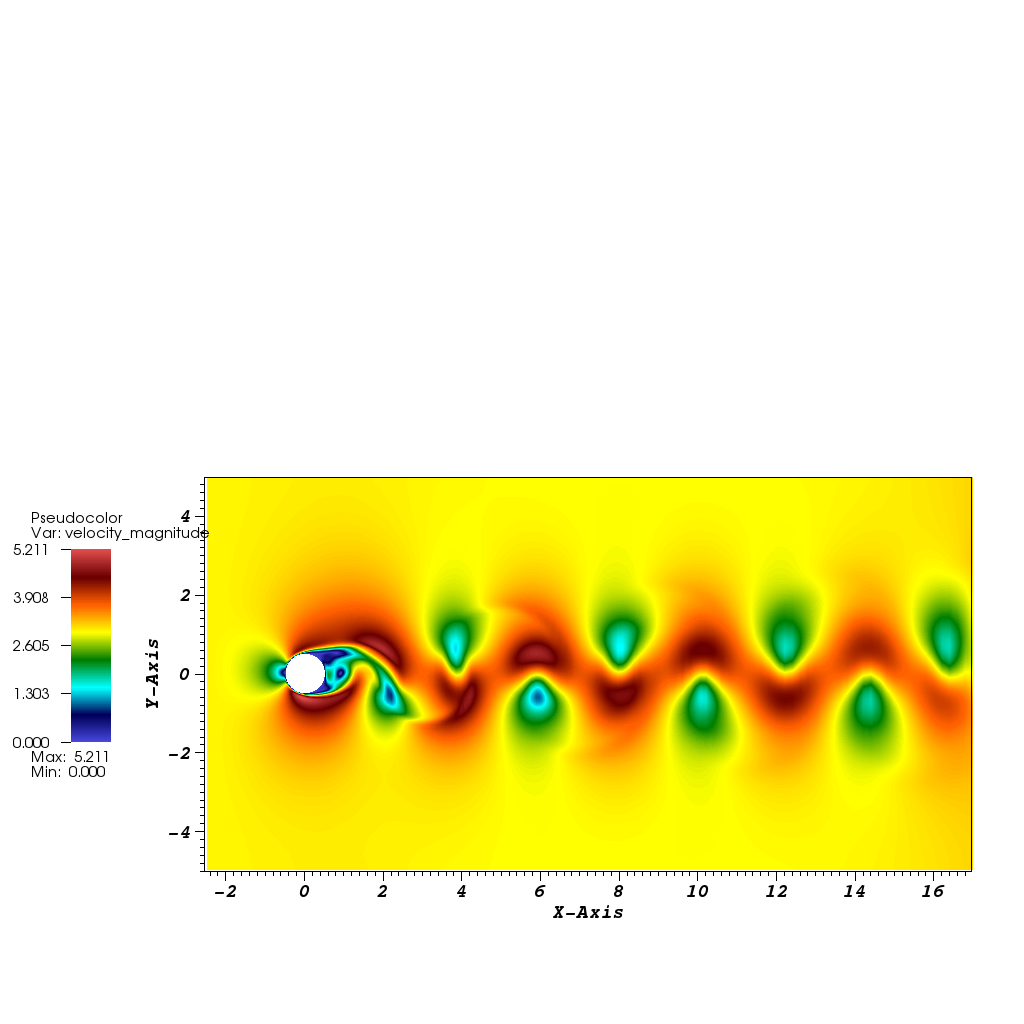
\includegraphics[width=\textwidth]{anchor_2/visit0016}
         \caption{FOM, $u=3$}
         \label{fig:6_b}
     \end{subfigure}
     \hfill
     \begin{subfigure}[b]{0.3\textwidth}
         \centering
         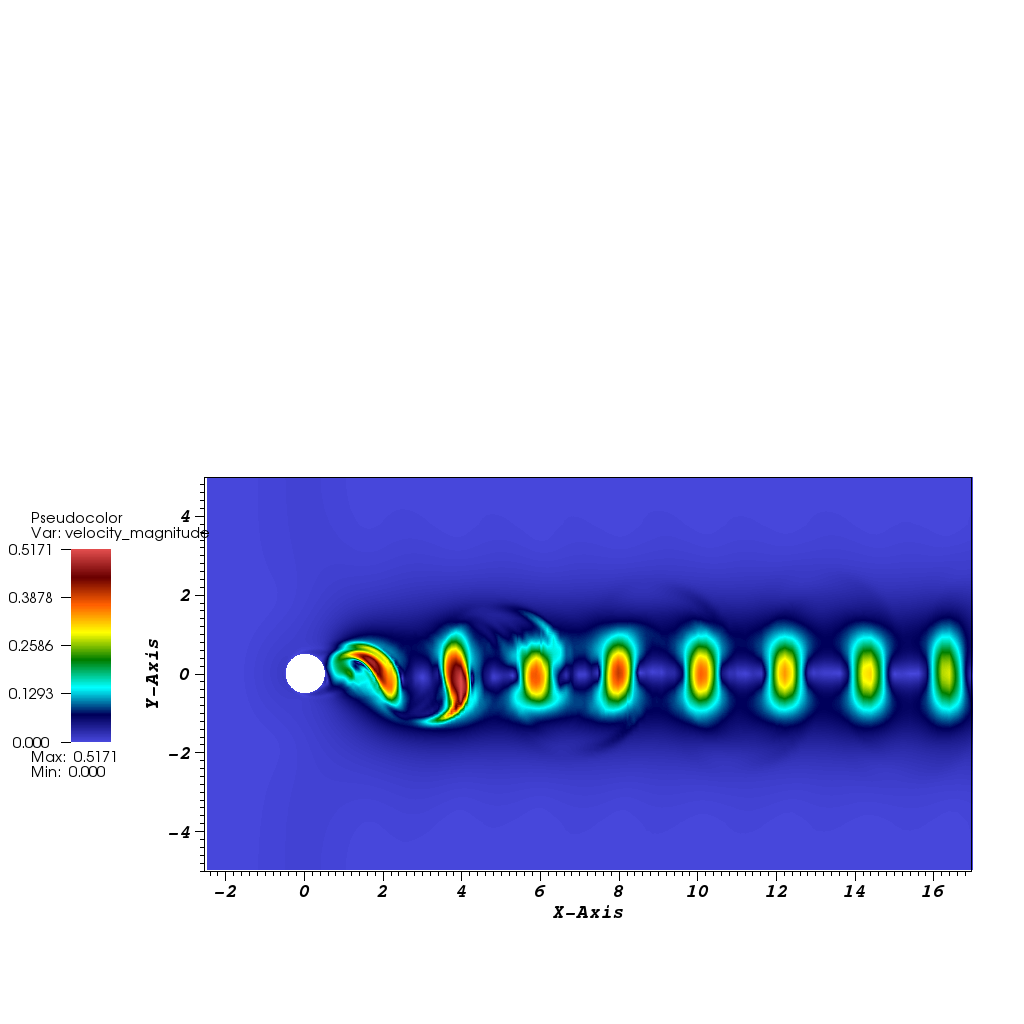
\includegraphics[width=\textwidth]{anchor_2/visit0017}
         \caption{Difference, $u=3$}
         \label{fig:6_c}
     \end{subfigure}\\
     \begin{subfigure}[b]{0.3\textwidth}
         \centering
         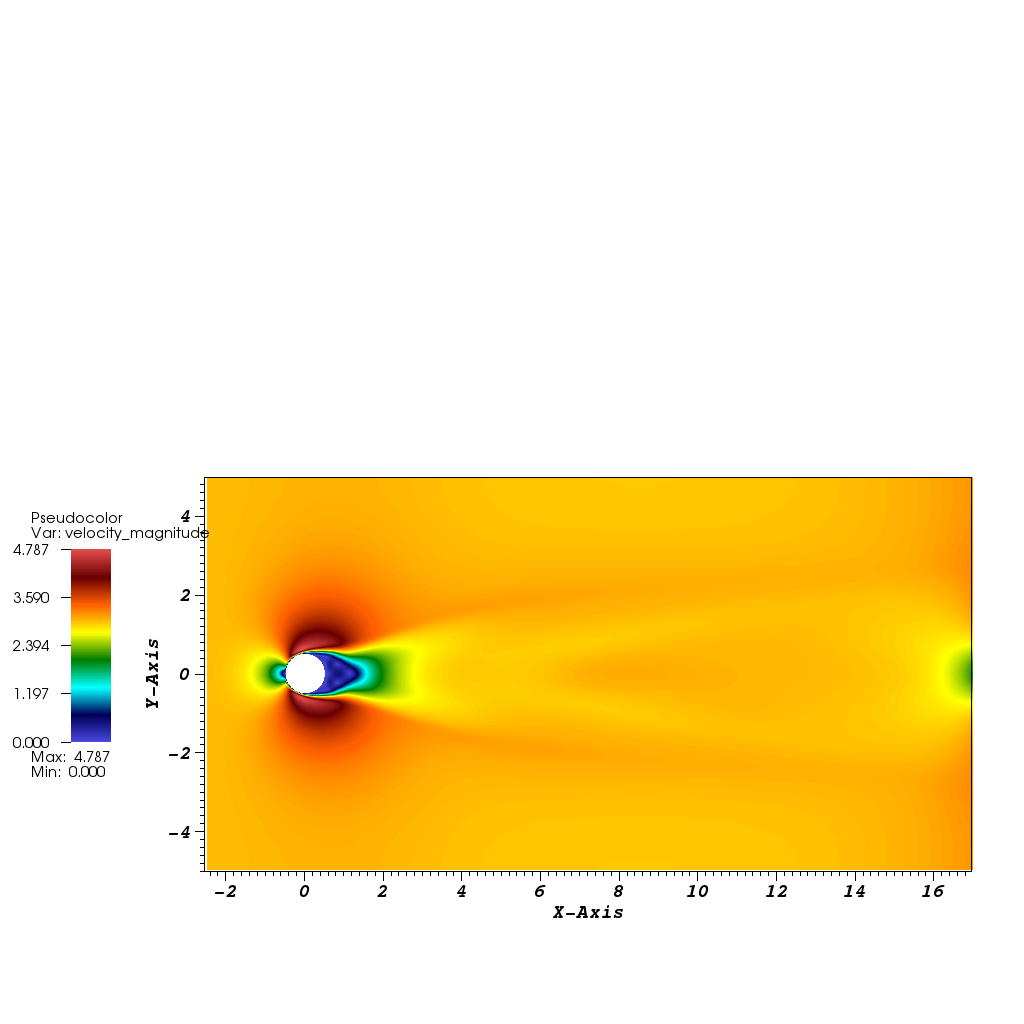
\includegraphics[width=\textwidth]{anchor_2/visit0019}
         \caption{ROM, $u=3$}
         \label{fig:6_d}
     \end{subfigure}
     \hfill
     \begin{subfigure}[b]{0.3\textwidth}
         \centering
         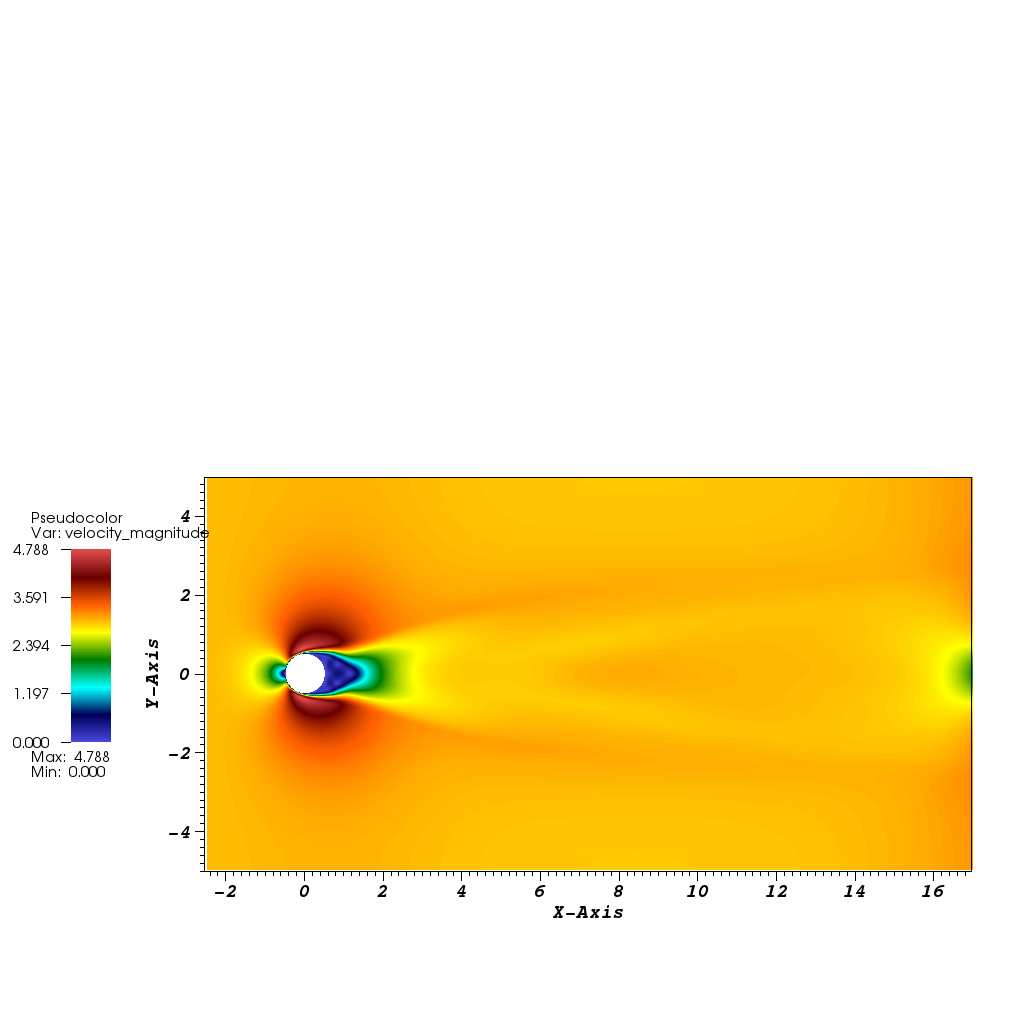
\includegraphics[width=\textwidth]{anchor_2/visit0020}
         \caption{FOM, $u=3$}
         \label{fig:6_e}
     \end{subfigure}
     \hfill
     \begin{subfigure}[b]{0.3\textwidth}
         \centering
         \includegraphics[width=\textwidth]{anchor_2/visit0021}
         \caption{Difference, $u=3$}
         \label{fig:6_f}
     \end{subfigure} 
     \caption{\subref{fig:6_a}--\subref{fig:6_c}: Solution comparison between
     ROM and FOM and its difference at $t=250$. Maximum difference $\approx 0.5$.
     \subref{fig:6_d}--\subref{fig:6_f}: Averaged solution comparison between
     ROM and FOM and its difference. Maximum difference $\approx 0.007$.}
      \label{fig:6}
\end{figure}
